\documentclass[onecolumn, draftclsnofoot,10pt, compsoc]{IEEEtran}
\usepackage{graphicx}
\usepackage{url}
\usepackage{setspace}
\usepackage{pdfpages}
\usepackage{listings}

\usepackage{geometry}
\geometry{textheight=9.5in, textwidth=7in}

% 1. Fill in these details
\def \CapstoneTeamName{Transportation Modeling}
\def \CapstoneTeamNumber{43}
\def \GroupMemberOne{Eytan Brodsky}
\def \GroupMemberTwo{Liang Du}
\def \GroupMemberThree{Samantha Estrada}
\def \GroupMemberFour{Shengjun Gu}
\def \GroupMemberFive{Charles Koll}
\def \CapstoneProjectName{Autonomous vehicle routing in congested transportation network.}
\def \CapstoneSponsorCompany{Oregon State University}
\def \CapstoneSponsorPerson{Haizhong Wang}

% 2. Uncomment the appropriate line below so that the document type works
\def \DocType{Project Hand Off}

\newcommand{\NameSigPair}[1]{\par
\makebox[2.75in][r]{#1} \hfil 	\makebox[3.25in]{\makebox[2.25in]{\hrulefill} \hfill		\makebox[.75in]{\hrulefill}}
\par\vspace{-12pt} \textit{\tiny\noindent
\makebox[2.75in]{} \hfil		\makebox[3.25in]{\makebox[2.25in][r]{Signature} \hfill	\makebox[.75in][r]{Date}}}}
% 3. If the document is not to be signed, uncomment the RENEWcommand below
%\renewcommand{\NameSigPair}[1]{#1}

%%%%%%%%%%%%%%%%%%%%%%%%%%%%%%%%%%%%%%%
\begin{document}
\begin{titlepage}
    \pagenumbering{gobble}
    \begin{singlespace}
        %\includegraphics[height=4cm]{coe_v_spot1}
        \hfill
        % 4. If you have a logo, use this includegraphics command to put it on the coversheet.
        %\includegraphics[height=4cm]{CompanyLogo}
        \par\vspace{.2in}
        \centering
        \scshape{
            \huge CS Capstone \DocType \par
            {\large\today}\par
            \vspace{.5in}
            \textbf{\Huge\CapstoneProjectName}\par
            \vfill
            {\large Prepared for}\par
            \Huge \CapstoneSponsorCompany\par
            \vspace{5pt}
            {\Large\NameSigPair{\CapstoneSponsorPerson}\par}
            {\large Prepared by }\par
            Group\CapstoneTeamNumber\par
            % 5. comment out the line below this one if you do not wish to name your team
            \CapstoneTeamName\par
            \vspace{5pt}
            {\Large
                \NameSigPair{\GroupMemberOne}\par
                \NameSigPair{\GroupMemberTwo}\par
                \NameSigPair{\GroupMemberThree}\par
                \NameSigPair{\GroupMemberFour}\par
                \NameSigPair{\GroupMemberFive}\par
            }
            \vspace{20pt}
        }
        \begin{abstract}
        % 6. Fill in your abstract
            This document contains all information regarding the "Autonomous vehicle routing in congested transportation network" project. It is a record of the progress of the project over the course of the year.
        \end{abstract}
    \end{singlespace}
\end{titlepage}
\newpage
\pagenumbering{arabic}
\tableofcontents
% 7. uncomment this (if applicable). Consider adding a page break.
%\listoffigures
%\listoftables
\clearpage

% 8. now you write!
\section{Introduction to Project}
Our project was requested by Dr. Haizhong Wang, a professor in OSU’s Civil and Construction Engineering department.
Dr. Wang does research in traffic flow modeling and simulation, as well as agent-based modeling and simulation for transportation network efficiency.
With the expected increasing number of autonomous vehicles in the world and with the inclusion of autonomous vehicles into transportation network models, it is important to explore how they will coexist with human driven vehicles, and if it is possible to improve transportation network efficiency by having both human driven and autonomous vehicles coexist in the same network.
Our team members are Charles Koll, Samantha Estrada, Shengjun Gu, Liang Du and Eytan Brodsky.
\newpage
\section{Requirements Document}
With the inclusion of autonomous vehicles into transportation network models, the method of how they will create optimal paths is questioned as well as how they will coexist with human driven vehicles.
To address this issue, we intend to investigate the integration of connected autonomous vehicles (CAVs) and gain data suggesting that vehicle autonomy and the overall infrastructure of transportation may be restructured positively to include multiple intelligent agents.
Additionally, this project will use a Python based framework and vehicle models to create data on how CAVs behave on a transportation network.
\begin{table}[h]
\caption{Updates Since Draft 2}
\begin{tabular}{|l|p{2in}|p{2in}|}
\hline
Section                  & Original  & New \\ \hline
System Functions         & includes requirement to compile data for a given vehicle's trajectory selected by a user                               & requirement changed to collect and show average data for all vehicles                                                          \\ \hline
Functional Requirements  & includes requirement to have functionality for reaction times for HV's and including "other traffic signs" as a factor & requirement will have functionality for vehicle reactions to factors such as other vehicles and traffic lights                 \\ \hline
Performance Requirements & describes system being able to support tens of thousands of vehicle models                                             & remove requirement, add that each vehicle should correctly and independently adjust its speed based on the car it is following \\ \hline
System Interface         & user should be able to check status and change each parameter                                                          & user will be able to interact with the GUI by building the simulation, pausing, playing, replaying, and zooming in             \\ \hline
System Mode and States   & includes that user will begin simulation by "start" or "run"                                                           & user will begin simulation with "build"                                                                                        \\ \hline
Environmental Conditions & the program will run on Linux systems                                                                                  & the program will run on Ubuntu systems                                                                                         \\ \hline
Information Management   & the user should be able to record and save simulations                                                                 & remove requirement                                                                                                             \\ \hline
\end{tabular}
\end{table}
\subsection{Introduction}
\subsubsection{System Purpose \& Scope}
The purpose of this project is to provide a framework and interface to simulate the behaviors of connected autonomous vehicles in a transportation network, represented as a grid network.
With this framework, models of autonomous vehicles will be created to participate in the simulation, allowing researchers to derive data on their contribution to traffic congestion.
\subsubsection{System Overview - System Context}
This system will be used in a research environment to observe autonomous vehicles and their behavior.
The data compiled from the simulations run on this system will be relevant to transportation infrastructure research and observation.
\subsubsection{System Overview - System Functions}
This system will create a city transportation grid world to simulate autonomous and human driven vehicles on a Python based framework.
A simulation will be run by an input of vehicle data, including information such as what the vehicle’s type is, its acceleration, and whether it is autonomous or human driven.
Taking this data, a gridworld will be built, and vehicles will attempt to route to their destinations using a simple Dijkstra’s algorithm.
After a simulation is run, it will provide precise data for users that includes each vehicle's id, start and end locations, speed, and direction.
The user may adjust the transportation system before each simulation, controlling the amount of CAV’s active and the number of vehicles overall.
This functionality is intended to be integrated with a GUI that will display the simulation in a playable and interactive format.
\subsubsection{System Overview - User Characteristics}
Target users will be limited to researchers interested in transportation infrastructure, all able to navigate through the interface and understand the results of each simulation.
\subsubsection{Definitions}
\begin{itemize}
\item CAV - Connected Autonomous Vehicle.
\item HV - Human-driven Vehicle.
\item GUI - Graphical User Interface.
\item API - Application Programming Interface.
\end{itemize}
\subsection{References}
\begin{itemize}
\item Ying Liu, Lei Liu and Wei-Peng Chen. 2017. Intelligent Traffic Light Control Using Distributed Multi-agent Q Learning. arXiv:1711.10941v1 [cs.SY]
\item Rick Zhang, Federico Rossi and Marco Pavone. 2016. Routing Autonomous Vehicles in Congested Transportation Networks: Structural Properties and Coordination Algorithms. arXiv:1603.0093v2 [cs.MA]
\item Alireza Mostafizi, Mohammad Rayeedul Kalam Siam and Haizhong Wang, Ph.D. 2018.  Autonomous Vehicle Routing Optimization in a Competitive Environment: A Reinforcement Learning Application.
\end{itemize}
\subsection{System Requirements}
\subsubsection{Functional Requirements}
The project should give an accurate simulation of traffic under conditions specified by the user.
These conditions will be parts of a traffic environment such as infrastructure layout, vehicle types (connected autonomous vehicles and human-controlled vehicles), vehicle starting locations, and vehicle destinations.
The project should accurately simulate interactions between the environment and autonomous/human-controlled vehicles, taking into account factors such as acceleration, speed limits, and traffic lights.
\subsubsection{Usability Requirements}
To make this a usable interface for testing traffic routing and simulation, we will need to develop an intuitive GUI.
Through this GUI, the user should be able to specify the number, position, and other parameters of variables in the environment.
These will include vehicles, road layouts, traffic signals, and speed limits.
The user should be able to simulate different conditions, pause, play and replay the simulation at any time.
\subsubsection{Performance Requirements}
This system is required to be able to display to the user at a minimum of ten frames per second.
Each vehicle has an independent estimation about its optimal route.
By connections between vehicles, they will know conditions about roads around them and each vehicle should respond to a vehicle that they follow, to prevent collisions.
All of these vehicles will have different destinations.
A metric to be used will be the average travel time of each agent.
\subsubsection{System Interface}
There will be a usable API in the server-side code.
By modifying the JSON file that is used as input for the vehicle layout, the user may change parameters such as each vehicle's type (CAV or HV) and their source and destination.
After a simulation completes, it has the option to be replayed if the user wishes, or they may begin again with new data.
During the course of a given simulation, a user may also zoom in to wherever their cursor is on the interface to get a close and clear look at vehicles, roads and intersections.
\subsubsection{System Modes and States}
The program will have a start state of an empty grid representing a transportation network, with which the user will begin their interaction.
From here, the user may manipulate the number or percentage of automated vehicles to the amount of human driven vehicles, along with beginning locations of each vehicle.
They may then enter the simulation state by pressing "build".
The simulation will run, and then display a playback of what occurred.
The user will then be able to pause, play, replay or zoom into the simulation or re-run with different parameters.
\subsubsection{Environmental Conditions}
The program will run on Ubuntu systems.
If there is enough time we can consider writing a version that works on Windows, but Ubuntu makes it easier to run and test on available hardware.
We will use Python to edit program structure.
Then we will use JavaScript to visualize it.
We will separate the program into three files.
\subsubsection{System Security}
Security is not a major requirement for this project, since there are no network connections going outside of the local network.
Without access to the physical machine, there is no risk, and even with access to the local machine there is no sensitive information in the application.
\subsubsection{System Life Cycle Sustainment}
The system will be developed until mid-March, at which point it will be in its useful phase.
Starting in June, unless a group decides to maintain the software, it will enter its legacy phase.
It will potentially be decommissioned if another group develops a more effective product.
\subsection{Final Gantt Chart}
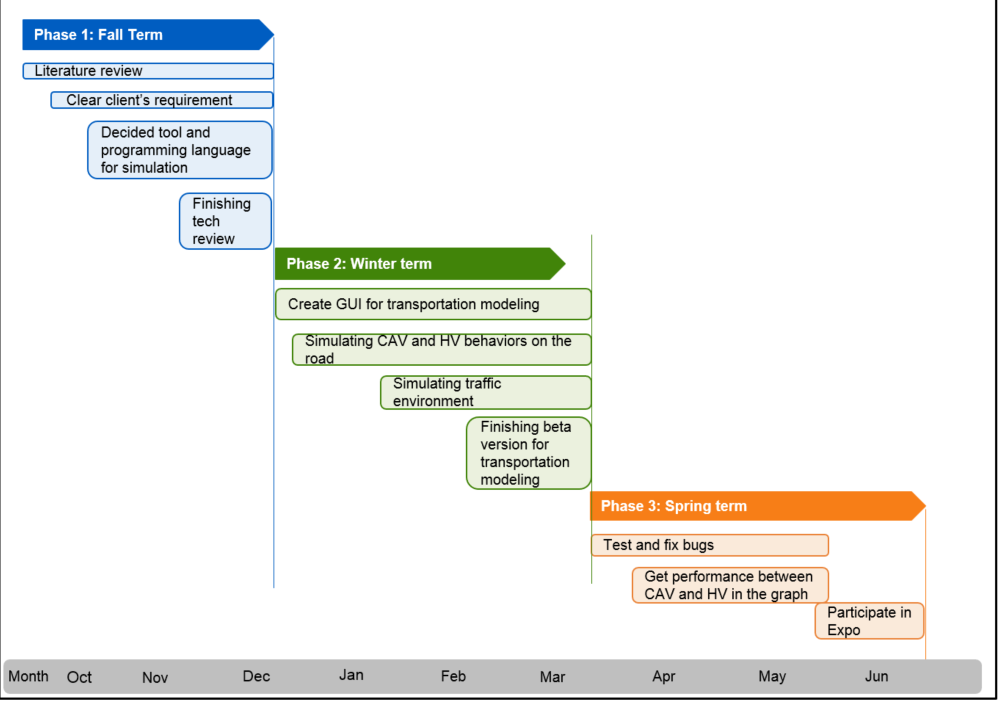
\includegraphics[width=6in]{ganttchart}
\newpage
\section{Design Document}
The purpose of this document is to make design choices for building a connected autonomous vehicle model and provide a structure of a CAV simulation.
This document discusses details of functionalities of the CAV model in each component and shows design choice reasons for each component in the design rationale and ways to complete each component in the design viewpoint.
\begin{table}[h]
\caption{Updates Since Draft 1}
\begin{tabular}{|p{1in}|p{2.5in}|p{2.5in}|}
\hline
Section                                         & Original  & New \\ \hline
Purpose                                         & simulate effect CAVs have on congestion & simulate effect CAVs have on overall transportation network \\ \hline
Testing                                         & road testing will include both one way and two way modeling; simulation playback will replay a saved video by the user & remove one way modeling; add that traffic light transition time is currently set at every 10 frames; simulation playback will simply replay last run simulation \\ \hline
Infrastructure                                  & one way and two way roads; each vehicle has a different reaction time; CAV algorithm uses connectivity to route & remove; CAV uses altered algorithm that recalculates every time it approaches new intersection \\ \hline
GUI Design Viewpoint                            & user may be able to pause simulation to gather additional information & remove gather additional information \\ \hline
Vehicle Decisions and Modeling Design Viewpoint & functionality for CAVs to use connectivity of other CAVs; each vehicle will have a set of nearby vehicles whose optimal routes it will consider when formulating its own optimal route & functionality for vehicles to use speed, direction, and acceleration to decide its own for car following; each vehicle will have a set of nearby vehicles \\ \hline
Vehicle Viewpoint                               & vehicle connection range & each autonomous vehicle will reroute itself at every intersection, while each human vehicle will only route itself once at the beginning to determine its optimal path. Both HVs and CAVs determine their speeds based on the cars directly in front of them. \\ \hline
Vehicle Viewpoint                               & the vehicle will be modelled as a point on a graph, where the graph is a simplified version of the map. Each vehicle will have associated with it a speed, starting location, destination, and type (autonomous or not autonomous) & the vehicle will be modelled as a point on a graph, where the graph is a simplified version of the map. Each vehicle will have associated with it a speed, starting location, destination, entry time and type (autonomous or not autonomous) \\ \hline
Vehicle Viewpoint                               & vehicle communication & remove \\ \hline
Vehicle Viewpoint                               & to track performance, each vehicle will have metrics such as time on the road, distance travelled, time spent not moving, time spent significantly below the speed limit, etc. to test the effectiveness of this network of autonomous vehicles & to track performance, each vehicle will have a velocity metric to test the effectiveness of this network of autonomous vehicles \\ \hline
Design Rationale                                & DSP with regards to connecting vehicles & remove \\ \hline
Design Rationale                                & examples include starting, location, type and speed (average, most common, etc.) & examples include starting, location, type, entry time and speed (average, most common, etc.) \\ \hline
Testing                                         & both one-way lane and two-way lane hybrid modeling & remove \\ \hline
Testing                                         & for example, if the user sets the parameter beyond the limit value, the program will report an error "setting parameter is not accepted" & remove \\ \hline
\end{tabular}
\end{table}
\subsection{Introduction}
\subsubsection{Purpose}
The purpose of this project is to provide numerical data by simulating the effect autonomous vehicles will have on a transportation network.
By creating models of these connected autonomous vehicles (CAV), we intend to study the way these models react and coexist with other models representing human driven vehicles.
\subsubsection{Scope}
With this project, we hope to deliver a working simulation of autonomous vehicle models onto a transportation network, rendered onto a GUI for the user to see.
Additionally, we aim to create relevant and insightful data of autonomous vehicle trajectory and how overall addition of these vehicles affects the transportation infrastructure.
\subsubsection{Context}
The vehicle is evolving into a mobile platform that can communicate and connect with others.
Communication technology upgrades ceaselessly and progresses rapidly.
With the continuous upgrading of urban scale and road planning, the research on autonomous vehicles reflects their social value.
Easing congestion and road safety have become particularly important.
The vehicle navigation system and other electronic navigation products have been unable to meet the needs of modern society.
The development of autonomous vehicles is extremely urgent.
The concept is to integrate relevant sensing technology, communication technology, and autonomous control technology into the vehicle, so that each vehicle can choose the optimal path to its destination freely.
From the perspective of society, safety and convenience are important concerns of autonomous vehicles.
\subsection{References}
\begin{itemize}
\item Ying Liu, Lei Liu and Wei-Peng Chen. 2017. Intelligent Traffic Light Control Using Distributed Multi-agent Q Learning. arXiv:1711.10941v1 [cs.SY]
\item Rick Zhang, Federico Rossi and Marco Pavone. 2016. Routing Autonomous Vehicles in Congested Transportation Networks: Structural Properties and Coordination Algorithms. arXiv:1603.0093v2 [cs.MA]
\item Alireza Mostafizi, Mohammad Rayeedul Kalam Siam and Haizhong Wang, Ph.D. 2018.  Autonomous Vehicle Routing Optimization in a Competitive Environment: A Reinforcement Learning Application.
\end{itemize}
\subsection{Infrastructure}
\subsubsection{Design Viewpoint}
Infrastructure components help CAVs (Connected autonomous vehicles) operate in a simulation with less abstractions from the real world.
They restrict how vehicles travel.
Users can also easily collect data from infrastructures.
There are three main infrastructure components in the simulation: intersections, roads, and vehicles.

Intersections are set up to connect roads together.
For each intersection, traffic lights turn “green” (allow vehicles to pass) and turn “red” (don’t allow vehicles to pass) alternatingly.

Roads connect intersections together and let vehicles drive on them.
Road settings make all vehicles clarify where they can drive on a map.
They are also convenient to collect data of each vehicle on the map; a user can easily know each vehicle’s location.

There are two types of vehicles in the CAV model.
One is the HV (human driven vehicle) and another is the CAV (connected autonomous vehicle).
Human driven vehicles are used to compare with CAVs.
Both types of vehicles have location and decision moves.
Location describes each vehicle’s position through the x and y axes (although one could use the z axis to represent height).
It is easy for the user to track a given vehicle.
For connected autonomous vehicles, the move decision is based on an algorithm which calculates its route every time it approaches a new intersection.
For human-driven vehicles, the decision move action is based on the route that has been set up at the beginning.
\subsubsection{Design Rationale}
The CAV simulation needs to simulate the real environment, but not all infrastructures in the real world should be built into the simulation because some infrastructure components do not influence vehicles’ driving (buildings, persons, etc.).

The infrastructure portion of the simulation provides basic rules for vehicles driving.
Intersections can show vehicles’ behaviors when they intersect.
Since roads are the carriers of vehicles, the infrastructure decides vehicles’ driving direction.
Connected autonomous vehicles are the main research object, and the performance of connected autonomous vehicles in a simulated traffic network determine its ways of communicating and the algorithm for selecting a route.
To judge connected autonomous vehicles’ performance driven on the road, human driven vehicles are used as a judging criterion.
One of the advantages of just simulating these three infrastructure components is making traffic network easier to operate and analyze.
\subsection{Graphical User Interface}
\subsubsection{Design Viewpoint}
The graphical user interface (GUI) will consist of a website page that has a section for setting parameters of the simulation and a section for viewing the actions of the simulation.
To use the GUI, the user will start by choosing parameters that they want the simulation to use.
After doing so, they will then press a button that will start the simulation.
When the simulation completes its computations, the GUI will then display the actions that the simulation took when it ran.
The user will be able to pause and resume the display.
When they decide to run another simulation, they can adjust the parameters and press the button that starts the simulation.

The graphical user interface will interact with the simulation backend in the following ways.
Upon startup, the GUI will establish a websocket connection with the simulation backend.
Once the user has chosen the parameters and pressed the button, the GUI will send the parameter information via the websocket connection to the simulation backend.
The backend will then run the simulation with the data it has been given.
Upon completion of calculating a single frame of the simulation, the backend will send the updated points of every entity to the GUI, which will store this information.
The backend will continue this process for every frame of the simulation.
Once it completes the simulation, it will send a termination frame to the GUI, which will specify that the simulation has been completed.
When the GUI receives this frame, it will alert the user.
Using the data gathered, the GUI will render it to the screen, displaying the actions like a video.
It will use WebGL to render the data to the screen.
\subsubsection{Design Rationale}
The graphical user interface will use websockets to connect to the simulation backend because it needs to keep a constant connection and pass large amounts of data.
The constant connection is required because of the large amounts of data.
If the backend were to pass all of its simulation data to the frontend at a single time, that could potentially take several seconds or even minutes, depending on the stability of the connection.
Sending to the frontend during the computations of the simulation allows for that time to occur during another period of waiting.

The GUI renders the simulation asynchronously to the computations of the simulation.
This provides several advantages.
If the simulation takes a long time to run (possibly hours), this can occur without need of the GUI to maintain a connection.
It only needs to retain a connection for each frame to be sent.
If each frame takes minutes to compute, the sending time of the data from the frame is relatively small.
Another advantage is that the visual aspect of the simulation can appear to run at the same pace as reality.
That allows for many frames per second, appearing more smooth and like a video.
If each frame took several seconds to compute and it were rendered immediately following, it would be hard to understand the actions of various entities.

WebGL will be used to render the simulation for its capabilities in using the GPU (graphical processing unit) to quickly compute large numbers of entities at once.
Without WebGL, it could be very difficult if not impossible to render all of the entities enough times each second.
A possible solution could be to prerender the entire simulation and display it as a video, but that has some drawbacks.
On of these is that the user could not be able to interact with the video to gather additional information.
WebGL provides this functionality, while allowing for enough frames per second that the simulation will appear to move smoothly.
\subsection{Vehicle Decisions and Modeling}
\subsubsection{Design Viewpoint}
Vehicle decisions such as routing will be calculated using Dijkstra’s Shortest Path algorithm (DSP), minimizing distance between the two nodes each vehicle will be concerned with: the origin and destination.
Put on a grid network, the DSP will go further to include nodes representing intersections, calculating its minimum distance to its destination from each.
Further, each vehicle will make use of other vehicles near it, using the information regarding those vehicles' speed, location, and acceleration to adjust its own for safe car following.

The vehicle will be modelled as a point on a graph, where the graph is a simplified version of the map.
Each vehicle will have associated with it a speed, starting location, destination, and type (autonomous or not autonomous).
Each vehicle will also have a route, which is a set of edges on the graph that the vehicle considers at the time as “optimal”.
For purposes of communicating with other nearby vehicles in the case of implementing a more sophisticated routing method, each vehicle will have a set of nearby vehicles whose speed and direction it will consider if they are close enough to follow it, which it will use to decide its own speed and acceleration.
To track performance, each vehicle will have metrics such as time on the road, distance travelled, time spent not moving, time spent significantly below the speed limit, etc. to test the effectiveness of this network of autonomous vehicles.
\subsubsection{Design Rationale}
Using Dijkstra’s Shortest Path algorithm achieves our main goal of implementing a routing method that each vehicle can rely on to bring them to their destination autonomously.
While straightforward and simple, DSP offers us an algorithm that minimizes a cost (either time or distance).
By including both speed limit of a given road with the distance a vehicle is at from its next goal intersection, we create a more realistic cost based on time.
A vehicle also takes into account its decision before it changes its vehicle attributes to match what it has decided, in order to make sure an action is valid.

The initial model for vehicles will be simple, consisting of basic metrics and parameters that can be specified and viewed by the user.
Examples include starting, location, type, entry time and speed (average, most common, etc.).
As the project progresses, we will consider adding more features and more attributes to the model to provide a more complete understanding of interactions between autonomous vehicles.
\subsection{Testing}
For testing our project program we need to find all possible errors.
Based on this program, we will build a city model and add vehicles for them.
There is a backend program that needs to be tested and a frontend GUI that also needs to be tested.

For the backend program test, we need to find all possible function errors.
In this program, we have road modeling, vehicle modeling, crossroad modeling, and signal light modeling.
We are required to test whether the whole model meets our design requirements.

Firstly, for the road test, we want to check whether all the roads meet the requirements of the design.
The lane must have an obvious lane number and lane direction.
After modeling is complete, if there is no obvious modeling mark for the road, the program will prompt "the number or direction of the road is not marked".

For the crossroad test, it requires connecting the corresponding lanes.
An error will be reported if only one lane is connected to an intersection.
Traffic lights in the corresponding direction will be set at the intersection.
If there are no lights at an intersection, the system will report an error such as “the intersection does not set correctly” or “there is no signal light set at the intersection”.

Traffic lights require regular changes in the law of real-time transformation, such as every 30 seconds to change the color of the lights.
When we are modeling, we will check whether the traffic lights have the following characteristics: timing of transition time and two colors (red and green).
For purposes of our model, we have set our traffic light transition time at every 10 frames.

Finally, vehicle modeling requires that vehicles be labeled as human or autonomous vehicles.
Each has an independent ID.
If the vehicle is not marked as a Human Vehicle or an Autonomous Vehicle, the system will report an error "the vehicle (id) is not marked".

Next, we will check all the possible errors in the GUI.
In the GUI we will create a city model containing many roads and traffic lights, on which users can set parameters freely, such as the number of vehicles.
The user will be able to see the program running time.
The user will be free to see how the model is running, such as displaying the path of the vehicle.
There are six parts we need to test.
They are Communication, Missing Command, Syntactic, Error Handling, Calculation, and Control Flow.

Firstly, for Communication errors since we will provide users with a complete user interface, it requires that all menus, options, and buttons must be able to let users immediately understand its function.
For example, menus, vehicle number settings, start, pause, terminate programs, and so on must be clear.
Users can see if there are any errors on the GUI.

Next, for testing Command errors we will add test code for each command.
When there is a button which does not respond after the user clicks it on the GUI, the user will see the program report an error "the button has no corresponding function".
After the program is edited, we will test it ourselves several times to ensure that each option has its corresponding function.
For example, the start option will start running the program, and the stop option will stop the program immediately.

Thirdly, for Syntactic Error, all words visible on the GUI must be spelled correctly.
It can be visually checked from the GUI.

Fourthly, we need to check Error Handling.
On the GUI, all errors must be described clearly.
Simply showing "error" on the GUI is not allowed.
All errors must be clearly stated whether they are internal or user errors.
For example, if the user sets the parameter beyond the limit value, the program will report an error "setting parameter is not accepted".

Fifthly, we need to check the program Calculation.
We cannot test it on the backend program.
Using the GUI to check calculations is more efficient for our job.
Computing problems require that we have clear logic, correct formulas, correct data types (including units) for each item of data, and correct function calls.
On the GUI, the number of vehicles required to be displayed corresponds to the number of user settings.
For this reason, we can check whether the number of vehicles conforms to the set parameters by formula or vehicle ID.
Each data type must be identified, such as time, vehicle speed, and distance length.
For example, for time calculation we can first set the change of the vehicle within 1 minute, but control the speed of GUI operation to estimate the change after 1 hour and then compare the actual change with the estimation method.
If the situation is similar, the calculation results are consistent with the real situation.

Finally, we will check the Control Flow.
The results of the software's control flow must conform to its description.
For example, the start button will start running the program, the pause button will pause the program, and the playback button will play back the last run simulation.
This test can be verified by practice during the use of the GUI.
\subsection{Conclusion}
Using the design decisions detailed in this document, we aim to complete a series of simulations from which we can derive significant and meaningful data.
The simulations will compare the impacts of CAV vehicles on a traditional network infrastructure with human driven vehicles.
Additionally, we have considered the presentation of this data, resulting in our decision to utilize a GUI where we may show graphs and render the simulation as a video.
We intend for this information to be easily available to the user through a simple yet informative GUI and sufficiently detailed for purposes such as research and general traffic simulation.
\newpage
\section{Tech Review}
\subsection{Eytan Brodsky}
\subsubsection{Introduction}
My role in the project is a software developer.
The goal of my review is to explore techniques of routing, optimizing and using various machine learning algorithms to improve the quality of our system.
This project offers a practical solution to the inclusion of autonomous vehicles into transportation network models and discusses how they will not only create optimal paths but coexist with human driven vehicles.
By pairing connected autonomous vehicles (CAVs) with a Q-learning algorithm, vehicle autonomy and the overall infrastructure of transportation may be restructured positively to include multiple intelligent agents.
Additionally, this project will explore the impact of CAVs relative to transportation congestion, using a Python based framework and vehicle models to create data on how CAVs behave on a transportation network.
This project will define the problem that autonomous vehicles present in the infrastructure we have already built and live in, as well as consider how navigation among other intelligent vehicles will be handled.
\subsubsection{Routing Algorithms}
One of the key elements in this project is figuring out how to optimally route vehicles in order to minimize delay for vehicles to reach their destinations.
This is a combinatorial optimization and integer programming problem, and is a known problem in computer science asking "what is the optimal set of routes for a fleet of vehicles to traverse in order to deliver to a given set of customers?"
Changing this slightly to "...fleet of vehicles to traverse in order to get to a given set of destinations" and asserting that each vehicle has its own specific target, we get a problem that is equivalent to our own.

Determining the solution to this problem is NP-hard, since this is a combinatorial optimization problem and the size of the problem can be fairly large.
Because of this fact, most commercial solvers use heuristics to approximate an optimal solution.
There are several main approaches to calculating these based on shortest path algorithms.
These include Dijkstra's algorithm, A* search, geometric containers, and several others.
\begin{itemize}
\item
Dijkstra's algorithm for this problem would maintain a priority queue of vertices ordered by distance from the current location of a vehicle.
This would then calculate the shortest path through a typical DIjkstra's algorithm run for each vehicle and call that the overall optimal solution to the routing problem.
The running time of this algorithm depends on the priority queue used, and is O((V + A)logV) with binary heaps as an example.
An alternative, yet somewhat similar way to calculate a shortest path, is using the Bellman-Ford algorithm, which scans all vertices whose distance labels have improved after iterative runs.
Another alternative is the Floyd-Warshall algorithm, which computes the distances between all pairs of vertices in O(v3) time.
For larger graphs, this can be faster than Dijkstra's algorithm\cite{bast2016route}.
\item
A* search uses a heuristic using a potential function on vertices, which is a lower bound on the distance from a vertex u to a vertex t.
It's essentially a modified Dijkstra's algorithm where the priority of a vertex is calculated differently from a normal Dijkstra's algorithm run.
For road networks--which is our specific application-- we can modify the geographical distance between a vertex u and a vertex t by calculating it to be the distance divided by the maximum travel speed (or maybe the expected travel speed based on data) for a path.
However, the lower bounds generated through the potential function are not stellar, and the performance gain is negligible\cite{bast2016route}.
\item
Another technique is called geometric containers, which--similar to A* search-- is a goal-directed method.
It pre-computes for each edge in the map a set of vertices whose shortest path from the starting point begins with themselves individually.
More research needs to be done into this method, but a disadvantage of it is that its preprocessing requires an all-pairs shortest path computation, which is very costly\cite{bast2016route}.
\end{itemize}
\subsubsection{Libraries for Q Learning}
Implementing the Q learning algorithm from scratch is unnecessary, since there are numerous libraries and packages that already have optimized versions of this technique.
Some of these include even more reinforcement learning algorithms for different purposes and applications, so it would be wise to take advantage of these libraries.
\begin{itemize}
\item
One library is Tensorflow, which is one of the most popular machine learning and deep learning libraries for python, which is going to be our primary language.
Tensorflow is created by the Google Brain Team, and is very efficient with its reinforcement learning algorithms.
Other similar libraries are Caffe and PyTorch, which can also be used in Python after downloading and also have a high degree of success and optimization like TensorFlow.

What sets TensorFlow aside from the other frameworks is that TensorFlow focuses more on a deep-learning view of problems by thinking of neural networks as graphs.
Its design allows for more modularity, as it treats different nodes in the neural network graph as smaller objects of tensor operations, which makes it more scalable and easier to use.
An advantage of using Tensorflow is that there are many tutorials and explanations available, and it's a very well-documented framework.

Another advantage of Tensorflow over other frameworks is Tensorboard, which allows for easy visualization of neural networks.
Tensorboard allows you to display model graphs, plot scalars, visualize distributions and histograms, visualize images, visualize embeddings, and play audio--though that might not be relevant for this project.
\item
With Pytorch, there are some different advantages that are not found in Tensorflow.
PyTorch is very Python-specific, and is oriented towards research or if our non-functional requirements are not very demanding.
PyTorch has an easier debugging experience as well, which might come in handy when initially developing, training and testing a model for our autonomous routing system.
Another benefit is that those of us who have taken machine learning and data mining during Spring 2018 have experience using PyTorch to set up a neural network architecture and train a model from an assignment, so the learning curve could potentially be smoother.
Since PyTorch is much more heavily Python-related than any of the other frameworks and since our project focuses heavily on Python, it could be a viable choice for a framework.
\end{itemize}
Ultimately it doesn't really matter which choice we make with our machine learning library, since for the purpose of a prototype we're not going to encounter any significant differences between these libraries' different implementation of certain algorithms.
Since all of these libraries and frameworks are based in--or at least can be implemented in--Python, and since we should all be comfortable with Python, it's only a matter of choice.
We choose something like PyTorch or Tensorflow and work on our model in that framework for simplicity.
\subsubsection{Performance Boosting}
While Python is a very convenient and easy-to-use language, it comes at the cost of not being very efficient.
Normally, Python is used to design prototypes of software components which would then be rewritten into a more powerful language like C or C++ depending on the application.
In our case where we want to have essentially real-time routing of autonomous vehicles, we will need to squeeze out every single bit of performance and optimization out of our system to ensure optimal performance.
Some ways to do this are to just switch to C++, use Cython, or use a neural network inference optimizer.
\begin{itemize}
\item
Switching to C++ seems to be the easiest choice at first, but of course there is a tradeoff.
While C++ is closer to the hardware at its core but accessible and object-oriented, it's still not the easiest language in the world to use and can be a challenge when dealing with unfamiliar libraries.
Using Tensorflow--as an example-- would become more difficult as looking up documentation and tracing back code and debugging would become trickier and more convoluted, since C++ is either intentionally or unintentionally more convoluted by nature.
The benefits of this of course are faster performance and in our case where we're performing heavy computations to get optimal routes for autonomous vehicles, we need as much computational efficiency as possible.
A potential balance is to write the basis of the system in Python and then switch the core of the system to C++, but there are easier ways of handling compatibility issues.
\item
Cython is a solution that can combine the efficiency of C++ and the ease-of-use of Python.
It's a superset of Python that compiles to C, which can yield large performance boosts depending on our task.
For work that's bound by Python's native object types, the speedups won't be large, but for numerical operations or any operations not involving Python's internals, the performance gain can be very noticeable.
Assuming we decide on a deep Q-learning model, this will involve extensive matrix operations which are computationally expensive and would benefit from being done in C or C++ rather than having to be bottlenecked by Python's inefficient numerical operations.
Python code directly calls into C modules, which are either generic C libraries or C libraries build specifically for Python.
Cython generates C libraries that talk to Python's C internals, allowing bundling with existing Python code.
With Cython, we can begin with an existing Python application and make spot changes to code rather than rewriting the entire application from the start.
\item
Another approach that's less likely to be adopted but is still a viable option is to use a neural network inference optimizer.
By treating the image of the map with cars and intersection light patterns, we can use tools like Intel's OpenVINO--which is available partially in open source--to optimize our network's execution.
This uses features like Winograd convolutions and various accelerators and strategic precision reductions to increase performance and throughput of frames put into a deep neural network.
This can be used together with other optimization techniques such as Cython to boost the performance even further, but will likely not be necessary at the beginning stages of the project.
Once the autonomous vehicle routing system has been implemented, we can start looking at ways to optimize neural network throughput to increase real-time performance.
\end{itemize}
\subsubsection{Conclusion}
There are many factors to consider when creating a system to route autonomous vehicles.
Besides the obvious route calculation and somewhat subtle deep learning aspects that can be used to improve performance, optimization of our system is important to ensure proper functionality.
Fast matrix multiplications, fast computation and ease of development are extremely important in developing a functional system, and we need to look at some of the options available to create a smooth and clear development process.
\subsection{Liang Du}
This project offers a practical solution to the inclusion of autonomous vehicles into transportation network models and discusses how they will not only create optimal paths but coexist with human-driven vehicles.
By pairing connected autonomous vehicles (CAVs) with a Q-learning algorithm, vehicle autonomy and the overall infrastructure of transportation may be restructured positively to include multiple intelligent agents.
Additionally, this project will explore the impact of CAVs relative to transportation congestion, using a Python-based framework and vehicle models to create data on how CAVs behave on a transportation network.
This project will define the problem that autonomous vehicles present in the infrastructure we have already built and lived in, as well as consider how navigation among other intelligent vehicles will be handled.
To achieve the final simulation framework of an autonomous vehicle transportation network, first, we need to do some literature review which will provide some ideas and help determine using which tool and algorithm to build the simulation.
Then it is necessary for our team to make a plan to create a simulation scenario.
And the final step is finishing the complete simulation framework which also includes testing and debugging.
\subsubsection{What your team is trying to accomplish}
Some basic performance metrics to be used will include a document about developing algorithms, building methods regarding routing and re-balancing issues, and creating a new routing network to test if our algorithm is suitable for autonomous and manned vehicles to identify each other.
We will use those algorithms and methods to build a basic simulation of 3 various types of vehicles (HV, AV, and CAV) in a routing transportation network.
Based on those methods, the simulation of vehicles and routing transportation network will be built by some software and it will need to be fit for basic rules that enforce physics in the real world (for example, it is impossible for vehicles to pass through each other or instantly go from a stopped position to their final speed).
In addition, after finishing the simulation of vehicles and routing transportation network, the basic simulation framework should have enough features to be able to test the given models, show that some models were developed and tested, and show that the information was collected and documented.
\subsubsection{Literature review - Intelligent Traffic Light Control Using Distributed Multi-agent Q Learning \cite{liu2017intelligent}}
Description: For current technology (Internet-of-Things), traffic light can recognize motorized vehicles and automatic turn red light to green light in the way of existing motorized vehicles.
However, traffic light cannot recognize non-motorized vehicles, like a bicycle.
In this literature, it describes a method to make traffic light inroad to be more effective, which not only consider single crossroad’s vehicles, but combining whole traffic system crossroad’s vehicles, and each crossroad can communicate with each other.

Tech option 1.1: Collecting crossroad’s vehicles information from the camera into the database.
To detect queue length not only for the vehicle but pedestrian in every intersection, it needs to use some cameras.
Then collecting that information and storing them into the database.
A single crossroad will have its own database.
Each single crossroad database will communicate with each other through the internet of Things.
This tech is the first steps to build a traffic light system.

Tech option 1.2: Building the computation module (Q Learning) and use it to control traffic light.
Q learning as one of machine learning algorithm has already used for designing traffic light system because Q leaning can make a decision by model-free online fashion.
That traffic information will be collected by “tech option 1.1”.
In every crossroad, the local camera will only collect local data (vehicle queue length), and through those data, the traffic system can only calculate local optimize path.
In order to achieve the global optimization, computation module (Q Learning) will not only used in the local database but will use in the global database.
Through global computation module to determine every crossroad’s traffic light (which traffic light should be green, and which should be red) so that achieve average traffic efficiency to be optimal.

Tech option 1.3: Using Urban MObility (SUMO) to simulate microscopic traffic condition, and there is an API designed in SUMO, which is used to evaluate performance via online interaction to adjust the status of the traffic light.
In the literature, they used to map data from open-street Map, and based on the map of Sunnyvale, CA.
Through software Urban Mobility (SUMO), it computed total queue length in the whole traffic system depending on a different method of controlling traffic lights.
In this performance evaluation, through Q learning algorithm to control traffic lights in the whole system got minimal total queue length.
However, only testing the total length of the whole queue length is not enough to show the Q learning method is better than other methods.
Therefore, this literature compared other statistics to show the Q learning method is better than others.
The other testing statistic is about the total waiting time of vehicles.
The result in the literature shows that the Q learning method spend minimal waiting time and MARL method followed.
In order to better comparing each data in every method, it used a bar chart to build statistics.
As the final result, they conclude Q learning method which appear in this literature is the optimal solution for controlling traffic light so that minimal traffic congestion.
\subsubsection{Literature review - Developing CAV Capacity Modification Factors}
Description: Connected and automated vehicles have an important influence on mobility, safety, and the environment in future transportation systems.
As a leading disruptive technology, CAV is expected to shift traditional traffic composition, usher in new operational models, change traffic stream characteristics, and reshape the ways state DOTs and associated agencies plan, design and evaluate roadways (Hendrickson and Samaras, 2017).
But, most of the current existing transportation facilities cannot “accept” connected and automated vehicle in right way, like current traffic light cannot recognize whether a vehicle is human-vehicle or CAV.
In this literature, it described some methods to build a transportation module that allowing Human connected vehicle and connected automated vehicle.

Tech option 2.1: According to this paper, Dr. Wang and his team have developed an agent-based modeling and simulation platform to evaluate the mobility and safety impacts of connected and automated vehicles.
This agent-based modeling and simulation platform is based on a software – SimDrive, for this software, it can simulate different levels of the autonomous vehicle.
SimDrive software is based on JavaScript programming and it allows the research team to easily modify the autonomous vehicle behavior for testing.
Based on this technology, experiments could be conducted to determine human comfort and acceptance of different speed in a different level of CAV.
Because there exists some autonomous vehicle performance case which is unacceptable, SimDrive software belongs to predictive capacity modeling.

For our project, we also can also use that software to build our testing module.
And it can help us collect data in many different situations and through data to analyze autonomous vehicles’ influence for the human.

Tech option 2.2: the Building base capacity function for microscopic simulation and analytical modeling.
This paper uses microscopic simulation to collect data, then using those data to build the bar chart.
Through analyzing bar chart, the team got the result about capacity change under different penetration rates, platooning intensities, and traffic throughputs with different numbers of managed connected and autonomous vehicle lanes under different traffic volumes.
The tech provides a good analyzing way for our project.
When we have some methods to optimize autonomous vehicles path chosen, we can firstly build a module and collect data from module to analyze.
And using a bar chart to make data more intuitive.

Tech option 2.3: The agent-based modeling and simulation (ABMS) system, which is a tool to simulate real-traffic situations.
Compare to field experiments, the ABMS system has a lower cost.
ABMS system also can simulate human-involved systems because it can simulate drivers’ actions based on complex reasoning.
ABSM system will make a decision according to around environment and programmers’ pre-set for ABSM system.
In addition, the agent-based modeling and simulation system is flexibility, which means it can balance capturing the coordination of individual objectives in agents’ tasks.
In the current stage, the agent-based modeling and simulation system is known as one of the best ways to simulate the connected environment.

For our project, the agent-based modeling and simulation system is a good choice to build an environment module, because it can help us to build many different environment modules.
And due to those environment modules are closed to real-environment, the data from those modules is more reliably.
What’s more, it also can help us to analyze autonomous vehicles’ chosen in the different environment.
\subsubsection{Python Based Modeling Framework - Mesa}
Description: Mesa is a python-based modeling framework.
It uses some ways to help users to build their agent-based models, like through “spatial grids”.
To make users more intuitive to operate their models, Mesa provides a browser-based interface to visualize them.
In addition, there are some data analyzing tool designed in Mesa to help users collect and analyze data more convenient.

Tech option 3.1: Mesa is a good software for a modular framework for building, analyzing and visualizing agent-based models.
The agent-based model is a programming behavior which is through computer simulation involving many different entities’ actions and “communicates” with each other.
Mesa is modular, which means modeling, analysis, and visualization components are separated but needed to work together.
Those modules are separated into 3 categories:
The first category is modeling, which is about building modules by themselves, agent classes and a model that is a scheduler to determine some sequences for the agent’s actions and space for them to move around on.
The second category is analyzing.
It is a useful tool to collect data which are generated from models.
To adjust collect different data from models, users just need to change the parameter value.
And the final category is visualization, it uses a server based on the JavaScript interface to create and launch an interactive model visualization.

Tech option 3.2: Pandora is another useful tool to build our simulation framework.
Pandora is a modeling framework which aims to create, execute and analyze agent-based models in an efficient computing environment.
It has been used to execute the large-scale agent-based simulation.
Pandora also can deal with thousands of complex actions.
The users can choose to develop their code in Python (for fast prototyping) or C++ (complex models).
Interfaces of both versions are identical and share the same C++ base code (assuring compatibility and efficiency).

The framework created by Pandora has full GIS support to cope with spatial coordinate-related simulations.
The library also allows the researcher to design experiments which can change simulation through change their parameters.
It can be built by using C++ or Python.

Compared to Mesa software, Pandora can use for C++ or Python programming language, it has better compatibility.
Pandora can help users to build their models and provide data, but it doesn’t contain analyzing tool like Mesa.
So, it must ask users to use other tools to analyze data from Pandora.

Tech option 3.3: After building a module for the transportation system of the autonomous vehicle, we need to use some tools to deal with data from modules.
Numpy and pandas will deal with this.
Numpy and pandas are one of Python's package, they provide data processing method.
Users can import data from their modules and through Numpy and pandas to analyze their data.
One of the important advantages of Numpy and pandas is they can spend less time to handle big data than other ways in Python.
Therefore, Numpy and pandas will give more testing result in short time, which is helpful for users to analyze their data.
\subsubsection{Conclusion}
There are two literature review and one tech review in this paper.
In the first literature review, it shows some technologies to improve traffic light's intelligent.
The second literature review discussed some software which is used to simulate traffic network, and that software is also can be used in our project's simulation.
And in the last part of tech review, it introduced Mesa software to build our project simulation and analyzing.
Mesa also was compared with other simulation software like Pandora.
\subsection{Samantha Estrada}
With this review, my team and I aim to acquire insight as to which told will aid us in gaining positive results from the discussion of how they autonomous vehicles will create optimal paths as well as how they coexist with human driven vehicles.
As a researcher and developer, my role within the team will be to pair connected autonomous vehicles (CAVs) with a Q-learning algorithm, and we hope to identify vehicle autonomy and their behavior within the overall infrastructure of transportation, perhaps leading us to a conclusion that their inclusion is beneficial to traffic congestion.
Using a framework and vehicle models to create data on how CAVs behave on a transportation network, this project will define the problem that autonomous vehicles present in the infrastructure we have already built and live in.
\subsubsection{Agent Based Modeling}
Firstly, we must identify what we will need to build our means of agent based modeling.
We would like something both easy to use and easy to create a UI with later on if we are able to.
This framework sits at the foundation of our project, as it will be used to test our autonomous vehicle models in a grid network manner.
Our first reaction was to create a Python based framework for our agent based modeling.
There currently exists a framework, “Mesa”\cite{Mesa}, that is specialized to this exact usage.
This tool is also useful as it provides analysis modules to we can utilize to capture data collection for when our simulation models are run.
Additionally, it houses visualization modules, which we may use to create the UI if we reach that point by pairing it with JavaScript to render the model.
This may be a viable option if we come to a conclusion that we would like to use a framework that is already built for us, and this framework appears to be one that is versatile and malleable.
Referring to a piece of literature within our team, there is also a developed platform called “MAgent”\cite{MAgent}specifically created to handle a multitude of intelligent agents, as well as control the amount of intelligent agents active during a given simulation.
This seems useful to our project in the scope of assessing the threshold at which intelligent agents become beneficial or even detrimental to traffic congestion.
This platform uses network sharing, which is important to us as we would like the vehicles to be connected.
MAgent also provides a rendering capability with a sliding scope for simulations, run on a C++ engine, which appears effective when assigning states and attributes for each agent.
The interface itself is in python and all rewards, actions, and agent symbols can be manipulated using a description language the team who has built this platform has developed.
Based on a Boolean style description of events, this platform seems useful and straightforward for simple tasks that our vehicle models will be faced with.
However, it does seem that it will need a bit of modification, as it focuses on benefits that come from competitive “prey/predator” style simulations.
However, this model is interesting as it introduces the concept that agents can become more intelligent working in parallel, which is a concept we have touched on when discussing how connected these connected vehicles would or could truly be.
This platform offers an added insight as to how the agents involved would behave both individually as societally, which could be interesting to analyze, but not directly necessary at this point in time.
\subsubsection{Traffic Congestion Alleviation}
Secondly, we hope to introduce an effective and integrated method of alleviating traffic congestion.
While the purpose of this project is mainly to simulate and create a behavior of how each autonomous vehicle navigates in a normal traffic infrastructure, we are also interested in ways to use the vehicles to decrease the amount of traffic congestion.
One technique we may introduce is the implementation of adaptive traffic signal control, introduced in the literature “An Agent Based Learning Towards Decentralized and Coordinated Signal control”.
In this paper, it offers the inclusion of Q-learning controlled traffic signals, rather than the pre-timed optimized signal control popular today.
This inclusion of reinforcement learning into the traffic signals can offer a level of reaction not commonly used, where the signals themselves will respond to the fluctuations of traffic flow.
This creates a relationship between the signals and its environment to enable it to act as its own agent, in turn assessing an optimal mapping between states and actions.
This could be beneficial to our project specifically as we hope to create a system that works cognitively with its environment, using not only individual vehicle agents but the infrastructure as a whole.
This literature introduces some drawbacks as well, such as the fact that implementing a model such as this will create a massive set of possible number of states for each traffic signal.
Additionally, this paper offers 3 states that a traffic signal through.
The first state defines a point in time where vehicles are approaching the current “green” light direction and the current queue length of those at the “red” light direction.
This state holds a vector of N components, each component representing a “phase”; one vector component represents the maximum arrivals, while other components are the maximum queue lengths for a given lane.
The second state uses queue length to represent delay, creating a vector of N components of maximum queue lengths.
Lastly, the third phase represents the vehicle cumulative delay, which is determined by a vehicle’s total time spent in a queue.
This simplistic model could be useful to integrate as it will offer us another method of data collection to ensure autonomous vehicles will not experience a heavy delay when interacting with traffic signals.
If we do implement this model, it is possible that it could alleviate traffic congestion by prioritizing reward (low time delay) whenever and wherever possible.
With the use of these traffic signals, this paper also suggests a decentralized system in which each intersection represents its own system.
Therefore, it displays total reward as taking two points and summing all total cumulative delays of all vehicles in the current system, the assessing their difference.
Vehicles are defined as leaving the system when they cross the stop line.
Therefore, reward may be defined quantitatively as positive or negative.
Again, this type of reward analysis using traffic signals as a data collection device could be something useful in the system we will be building, as we are interested in the numerical data and the ability to assess autonomous vehicle’s performance in terms of congestion or traffic delay.
\subsubsection{Vehicle Routing Within Congestion}
Lastly, we intend to cater a routing algorithm to not only find the most optimal route but work beneficially in congested areas.
A literature review on the paper “Routing Autonomous Vehicles in Congested Transportation
Networks: Structural Properties and Coordination Algorithms”\cite{Routing:2016} offers the concept of re-balancing the vehicles to ensure given areas will not be overpopulated with intelligent agents.
Within this paper, the scenario is presented that the agents are providing a taxi type service, in which they re-balance themselves into regions of a given area in order to properly cater to service requests.
Our scenario is more individualized, as we seek to model privately owned autonomous vehicles.
Still, this topic of re-balancing raises an important point, as one method of avoiding congestion is simply to avoid a given area that is becoming overcrowded.
The algorithm proposed in the paper utilizes the same reinforcement learning we've seen and discussed before, using rewards such as fuel usage and maximum maintained speed to determine the cost of a given route.
If the cost of a given route is deemed more beneficial than another, the vehicle may choose to re-balance itself to that location, even if the distance is greater.
Re-balancing also provides the opportunity for congested areas to become clear, as the volume of traffic does not continue to pile up.
This is a viable point to include when we are considering how to build our algorithm, as we must add this factor of “faster” routes costing more when they are lacking the right traffic flow.
It is also important to define how our model will recognize when congestion is occurring.
This paper also introduces their own method of allowing their grid network to self-diagnose congestion as soon as it becomes apparent.
Using classical traffic flow theory, this model compares vehicle density on a given road with the free flow phase of traffic.
If the flow of vehicles on the road (determined by the product of vehicle density and speed) reaches a determined maximum, the vehicles travelling reduce their speeds and the road is flagged for congestion.
This is another important detail we must consider, as we wish for the vehicles to be connected and therefore share data on where and when congestion occurs so that they may avoid it.
\subsection{Shengjun Gu - Overview}
This project offers a practical solution to the inclusion of autonomous vehicles into transportation network models and discusses how they will not only create optimal paths but coexist with human driven vehicles.
By pairing connected autonomous vehicles (CAVs) with a Q-learning algorithm, vehicle autonomy and the overall infrastructure of transportation may be restructured positively to include multiple intelligent agents.
Additionally, this project will explore the impact of CAVs relative to transportation congestion, using a Python based framework and vehicle models to create data on how CAVs behave on a transportation network.
This project will define the problem that autonomous vehicles present in the infrastructure we have already built and live in, as well as consider how navigation among other intelligent vehicles will be handled.
\subsection{Shengjun Gu - tasks we are working on}
We intend to set up a simulation of a traffic network with vehicles that work as a system.
Each vehicle has a destination, and given the destinations and current positions of all the other vehicles, each vehicle will calculate the optimal path to minimize the travel time for all of the cars in the simulation given a set of constraints such as path, speed limit, etc.
With a higher number of cars, the number of constraints in the optimization problem grows to a point where it would simply take too long to calculate these decisions in real time.
This is where some heuristics will come into place to estimate a solution to what is a very non-convex problem.
In total, we now have three issues to consider.
First one is real-time delivery of data which would require specialized software and hardware such as a real-time kernel and a NIC with real time capabilities for the autonomous driving itself.
Second one is highly efficient approximation algorithm to find the optimal routing for all vehicles in the network.
We need to find at least one way to implement the necessary functions of these automated vehicle detection, or at least simulate these functions, to better understand the problem during the experiment.
Thirdly, by studying actual traffic data, we must verify our assumptions.
We also need to prove that the proposed algorithm is even better than the point-to-point rebalancing algorithm is real-time routing and rebalancing algorithm.
\subsection{Shengjun Gu - TECHs}
\subsubsection{Vehicle Internet}
Literature Review about: Multi-Agent Reinforcement Learning for Integrated Network of Adaptive Traffic Signal Controllers (MARLIN-ATSC).
The steady growth of the global population has led to traffic jams in some densely populated cities or regions.
With the development of society, Adaptive Traffic Signal Control technology (ATSC).
The technology has great power to solve the problem of traffic congestion.
The technology can be used to improve traffic congestion, mainly through real-time adjustment of signal timing, for example, by minimizing delays and making the lights respond quickly to improve traffic problems.
This is the idea of an efficient ATSC designed by a Multi-Agent Reinforce Learning method, which requires each controller to control all traffic lights at a single traffic intersection.
This paper introduces a Multi-Agent Reinforcement Learning (MARL) method, which is mainly used the adaptive traffic signal controller (MARLIN-ATSC).
MARLIN-ATSC control system provides autonomous learning of ATSC through the cooperative combination of enhanced learning method and game theory.
MARLIN-ATSC mainly has two main modes :(1) Independent mode, that is, each intersection controller runs independently, and each agent has its own controller.
(2) Comprehensive mode.
In this mode, the controller can coordinate adjacent intersection signal control.
This paper introduces how to use the mathematical modeling of traffic control problem as a stochastic control problem, and combines with the application of artificial intelligence technology, such as the reinforcement learning in game theory setting.
Also, this paper provides useful and inexpensive solutions to real life traffic congestion problems.
There are three main Technology in this article.

First of them is Agents learn strategies based on implementing one of two learning methods: MARLIN-IC and MARLIN-DC.
In MARLIN-IC, each agent estimates the model of the neighborhood strategy and updates its strategy with the estimated model.
Similar to Q learning, MARLI-IC updates the estimate value function (Q value) using the best response action, independent of the currently followed policy, which involves an exploratory operation.
Therefore, MARLI-IC is considered to be an iterative value algorithm with non-policy approaches, as agents try to improve strategies while following another strategy.
On the other hand, in marlin-dc, the agent first randomly selects the policy and then swaps it with the neighbor.
The agent uses this information to evaluate and improve policies.
Therefore, MARLIN-DC is seen as a strategy iteration algorithm with a strategy approach.
In this case, the broker's policy is updated based on the current policy.
Finally, during the agent's decision-making process, the joint policy from the learning process is given with the neighboring agent.

Next the paper introduced that Paramics is an adaptive traffic control system for evaluating significant intersections in downtown Toronto using observed traffic data.
Reinforce Learning is compared with Webster - based fixed time signal control and NEMA actuation control as a reference.
The results show that Reinforce Learning-based signal control system is superior to fixed time and excitation control methods in saving the cumulative delay of each vehicle.
Also, it was found that compared with fixed time or actuation control.
Reinforce Learning -based controls are more robust and achieve the same average latency regardless of the contours reached.
It concludes that Reinforce Learning is more effective in the signal control and more vivid in an overview of variable demand.
Compared with fixed time and start-up control, the average Reinforce Learning delay saves 52 percentage and 35 percentage, respectively.
This reflects strong adaptability of Reinforce Learning to traffic fluctuations.

Third one is by the network of five intersections of Paramics in the center of Toronto.
Compare the two operating modes, MARLIN-ATSC, standalone mode and integrated mode usage.
The results of the experiment.
1) the MARLIN-ATSC integration mode is always superior to its independent mode.
That is, regardless of the level of demand, the integration model saves more on average intersection delays and average route travel time.
2) find MARL-IN more compelling at high demand levels.
Experiments show that when overflows occur from an intersection to an upstream intersection, under the condition of highly saturated, it has more efficient coordination.
This means that the MARLIN-ATSC integration pattern can provide more reliable travel time, a performance indicator of equal importance for travel time.
It is more recommended to use the indirect coordination mechanism (MARL-IN) direct coordination mechanism (MARL-DC).
Because it can show similar performance, but it has faster speed and it spends shorter time.
\subsubsection{Vehicle data collect}
When people understand the concept of self-driving cars for the first time, most of them will intuitively understand system dependence on data of incredible.
For example, the vehicle needs to be in continuous communication with a position tracking satellite and be able to transmit and receive messages from other vehicles on the road.
Whether it's finding a destination or getting around unexpected obstacles, everyone knows that self-driving cars must continually absorb data from the outside world and often feed that data to advanced neural network algorithms to filter out meaning in real time.
Still, as surprising as those extroverts are, few realize that these vehicles may collect as much data from inside the car as they do from outside.
Advanced vehicle AI will watch Tomorrow's self-driving car passengers, and in many ways, ride quality and safety will depend on the vehicle's ability to interpret human wishes and needs.
Traditional cars may run on natural gas, but autonomous vehicles run on data they can mine from anywhere.
I found three main Technologies.

First of all, by creating a convolutional neural network and capturing the raw pixels of a single front camera, the technology can then apply the data directly to the direction control.
It turns out that this end-to-end approach is very powerful.
Autonomous vehicles can systematically learn to drive on roads with or without lane markings as well as on highways.
Convolutional neural networks are also tested in areas where visual guidance is unclear, such as parking lots and unpaved roads.
With a lot of systematic learning, autonomous vehicle internal components can be self-optimized to maximize overall system performance.
This is better than autonomous vehicles systematically learning human behavior to meet reasonable human standards.

Second one is using cheap multimode sensor fusion system.
The system uses commercially available equipment and can realize automatically data collection of road condition.
Detailed evaluation and enhancement of various technical methods and algorithms to overcome visual measurement distortion caused by the movement of the monitoring platform.
Fracture detection using laser line scan is studied.
However, infrared thermal imaging technology is used to identify defects on the surface of the site.
The system includes an RGB-d camera, a global positioning system, an accelerometer and a data acquisition module.
There is evidence that the technology in providing accurate quantity limitations existing pavement and its calculation error.
In order to be able to properly integrate data from multiple sensors, infrared thermal imaging technology synchronization time is needed to establish the consistency between the heterogeneous data.
In addition, the data synchronization is based on the timeline of each sensor and recorded by the corresponding data acquisition program.

Third one is using a probability method to locate 3-D laser radar scanner automatic vehicles.
The central principle of the algorithm is modeled by a Gaussian mixture of several kinds of the world.
Therefore, the height and reflectivity of the environment are used to analyze the road condition.
The 2-D grid structure is recommended.
All independent cell grids are accompanied by a gaussian mixture model: height and appearance, which can capture the distribution of reflectivity.
Through the raster version of the multi-resolution gaussian hybrid, the system can be searched efficiently.
In these mappings, the registration is implemented, using the universal ceiling situation to implement the fast branch and binding registration and live registration, guaranteed the optimal registration.
This allows the system to get real-time information.
\subsubsection{Correct positioning of the vehicle}
As we know, vehicle positioning is a key requirement for many safety applications.
Accurate vehicle position information in the right time to correct the pilot group of warning is very important.
Active safety systems are primarily directed to alert and intervention strategies for security crises.
It needs to be able to accurately locate vehicles and accurately assess safety threats.
Today's global positioning system and digital map not only provide information on the location of the vehicle, but also provide real-time road conditions, so that they become an important tool for vehicle positioning.
Today's vehicles can share their location information with other vehicles and traffic operations centers.
The progress of wireless technology has greatly increased the use of vehicle mapping technology for road safety.
There are also three main Technologies.

First one is using a novel algorithm which is presented by using a non-tracking Kalman filter, which includes a global positioning system, a multi-hypothesis mapping matching algorithm and a vehicle positioning system that integrates navigation system data.
This technique has proposed a new way to evaluate the multi-hypothesis mapping algorithm, and to propose a way to increase the accuracy of the location based on the way it should be feedback.
In multiple hypothesis graph matching algorithm, if the node number exponentially with time, you need a large amount of computing time and memory.
This technology is dedicated to reducing the number of hypothesized nodes, by suggesting a few ways to generate technology by improving the virtual node, and by modifying the branch of the multiple hypothesis tree, to eliminate or merge the redundant nodes.
The system can achieve higher precision through map matching feedback, which can save computing time and memory significantly.
The data calibration module USES UKF or navigation position prediction (DR) to update and calibrate vehicle status information based on GPS data quality.
Also, if feedback information is available, it can be used to improve vehicle status information further.
Then, the calibration information will go into the map matching module, where the map matching will make the position of the vehicle match a road in the digital map.

Second one is using a new GPS system Differential Global Positioning System (DGPS) which is now available.
By increasing precision, automatic vehicle location (AVL) can now be accurate to a specific road lane.
Lane level positioning provides a better development platform for many new intelligent transportation systems and some applications, such as better management of fleets on the road, lane level navigation and carrier-based vehicle traffic measurements.
It is important for that match precision and utilization of the digital network data development.
Through these two methods, it is possible to determine the vehicle traffic lanes at any time.
This technology will help a lot of transportation research.

Third one is using enhanced maps on the vehicle.
Enhanced maps should represent roads.
First, it is more complete than previous maps.
Second, more accurate than standard maps, it offers more comprehensive applications for road safety and Advanced Driver Assistance Systems (ADAS).
GPS is a key system in automotive applications, but it still has some limitations.
The mobile map can be used to mark the area on the map, so that the system can directly collect the road network and generate real-time geometric shape in line with the road network.
Most map providers use dedicated vehicles equipped with calibration sensors to collect and process information.
This can not only locate the vehicle, but also map all the road markings and signs around it.
Thus, the system can have automatic identification function to help automatic vehicle self-positioning and self-identification.
\subsection{Shengjun Gu - Conclusion}
The above technologies will provide network flow models for autonomous on-demand systems with capacity.
We will develop routing and rebalancing issues so that it can always rebalance vehicles without increasing traffic congestion.
We may use the network model to prove that rebalancing does not increase congestion.
We will develop a computationally efficient congestion aware routing and rebalancing algorithm.
That highlights the awareness of traffic congestion in the autonomous control strategy design and implementation of importance.
We will create a new routing network to test whether our algorithm is suitable for autonomous and manned vehicles to identify each other.
We will then create a smart system to help cars find the best routes to run in the city, thus saving time for vehicles.
And we're going to submit the results, give you the theoretical information about how the autopilot system can do the best thing.
Finally, we will present the research results in a research report, with our road model, code example, and some theoretical formulas.
For the success of the project, we need to submit complete code of various tests, submit test reports, and measure the best configuration of unmanned vehicles, including AI system, algorithm, etc.
If we can create an entirely new measurement system, it will be more perfect.
If not, we will have to make maximum optimization based on the existing system and propose an optimal environment for Autonomous Vehicles.
\subsection{Charles Koll - Overview}
With the inclusion of autonomous vehicles into transportation network models, there is little data on how they will create optimal paths as well as how they will coexist with human driven vehicles.
To address this issue, we intend to investigate the pairing of connected autonomous vehicles (CAVs) with a Q-learning algorithm backed by reinforcement learning, aiming to gain data suggesting that vehicle autonomy and the overall infrastructure of transportation may be restructured positively to include multiple intelligent agents.
Additionally, this project will explore the impact of CAVs relative to transportation congestion, using a Python based framework and vehicle models to create data on how CAVs behave on a transportation network.
\subsection{Charles Koll - Literature Review: Modeling Traffic Signaling}
An important aspect to transportation modeling is the network infrastructure.
That can involve street lengths, number of lanes, traffic direction, intersections, and more.
To generally represent those I will discuss GUI frameworks in section 3.
There can be additional computation behind the infrastructure as well.
For intersections, there are traffic lights that determine the flow of traffic in those nodes of the network.
Developing a model without any routing at intersections may be easier to implement, but it could cause significant differences in the model from the real world that could negate any potential information collected from the model, especially when modeling traffic flow and congestion.

There are three primary goals when attempting to model traffic signaling.
These are simplicity, efficiency, and realism.
With simplicity, there cannot be too much computation time involved in determining when to change signals.
If there is too much time taken to determine when to change, it is possible that the optimal time to do so occurs during the computation.
Another goal that is easier to compute is efficiency.
How quickly can vehicles make it through the intersection?
Often this is the main reason for modeling the signals.
The final goal is how realistic the modeling is.
It is great to have an efficient and simple model, but if it can never be implemented in the real world, then it is useless for modeling.
\subsubsection{An Agent-Based Learning Towards Decentralized and Coordinated Traffic Signal Control \cite{el2010agent}}
To avoid complexity, one solution is to have each traffic control signal act independently of each other.
This prevents complexity often found in multi-variable problems and allows for greater complexity at an individual basis.
To optimize efficiency, the authors created a reinforcement learning strategy using Q-learning and genetic algorithms.
The reinforcement learning allows for an intersection to adjust its timings based on what it has encountered before to better guess an optimal timing.
A common method for implementing this is Q-learning.
It allows for various times to have more weight than others, so the signal would be able to adjust its strategy for busier times of the day.
A downside to reinforcement learning is that it is only based on what the signal has encountered previously.
While this means that the signal will improve its efficiency over time, it also means it will have a harder time dealing with new scenarios.
An example of this would be a large sporting event or natural disaster.
The signal would not see the type of traffic patterns it can handle, so it would not be able to perform at its most efficient.
However, the next time it encounters a similar event it would be better able to gauge how to act.
To find more efficient solutions based on a given scenario, genetic algorithms are useful to provide novel possibilities.
They introduce various types of randomness that allow for adjustments to the current solution.
To verify how realistic this type of modeling is, the authors performed a real-life test on a physical intersection in the city of Toronto.
The model performed quite well, with an efficiency much greater than that of a pre-timed signal.
While this is promising for the efficacy of the model on a very small scale, it is difficult to determine how a network with many of its intersections fitted with this model would perform.
However, considering its efficiency and being relatively realistic, reinforcement learning with Q-learning is a promising possibility for our project.
\subsubsection{Multi-Agent Reinforcement Learning for Traffic Light Control \cite{wiering2000multi}}
The author used a slightly different form of modeling for their traffic control signals called model-based reinforcement learning.
While this is very similar to Q-learning, it differs in a couple of key points.
Model-based reinforcement learning requires less computational complexity and can learn more quickly from training data, but it requires discrete input data (time, vehicle locations, etc.) and takes more space.
This appears promising from the perspective of efficiency but less so from the perspective of reality.
While it seems that this type of training is a computationally easier route for modeling, it is unlikely that it would work in the real world due to it requiring discrete information.
Theoretically, inputs that are traditionally continuous could be translated into discrete inputs that function well for the signals.
However, that would likely require more computation and negate some of the benefit to its quicker learning.
Due to these reasons, I think it unlikely that this type of traffic control signal modeling would work well for our project.

It is interesting to note that both documents used reinforcement learning for the traffic control signals.
While the method may be a bit complex and require much training data before it is viable, it is hard to beat an efficiency that improves over time.
\subsection{Charles Koll - Literature Review: Distances Between Connecting Vehicles}
When considering connected autonomous vehicles, one must determine the extent of the connectivity.
Internal vehicle models can greatly increase in computational complexity as they take in more data about the vehicles around them.
While this complexity can lead to more efficient actions, if it is let to grow too large then it can hinder the responsiveness of the vehicle.
To solve this problem most models consider vehicles which can communicate with others in their immediate vicinity (those whose actions are most likely to impact the given vehicle), with a set of protocols in place to handle external factors.
\subsubsection{Connected Vehicles: Solutions and Challenges \cite{lu2014connected}}
A set of protocols must be able to handle external factors of the environment of transportation infrastructure.
Buildings and other objects can block signals between vehicles.
Distance can create latency on a connection and weak signals.
Differing velocities can change rates at which signals get passed back and forth.
All of these are challenges that the protocols must be able to handle.
The authors suggest several ways of handling these challenges, which pull from existing technologies in internet networking.
These include multiple antennas, frequency division multiplexing, and dynamic spectrum access.
The research proposes solutions to environmental challenges, but does not implement these in a model.
It is unlikely that any one model could handle the computational complexity to introduce all of these problems, but they are useful notes to consider when determining if a model is realistic enough.
\subsubsection{Game-Theoretic Control for Robot Teams \cite{emery2005game}}
As explained by the author, computational complexity for games where agents, in our case vehicles, must logically determine the actions of another often becomes intractable for just two agents, much less several.
This leads to their suggestion that data passed along the network between connected agents be just enough to optimize to a local maximum rather than global.
As noted in the previous research, network connections have their own problems of reliably passing information, so that provides another reason for passing minimal data and/or connecting to fewer vehicles.
A local maximum is unlikely to be much worse than a global one, and across many agents it could produce a more efficient solution overall.

For our models we will be sure to consider situations that would be unlikely to work in real-life scenarios and determine suitable workarounds so that they are realistic enough to potentially succeed in real-world testing.
\subsection{Charles Koll - GUI Frameworks for Modeling Transportation Infrastructure}
When developing models to represent vehicles interacting with a transportation infrastructure, it is useful to have a graphical interface to use for presenting results or testing code.
The component of the GUI that is used to represent the transportation infrastructure can be built from frameworks.
\subsubsection{tkinter \cite{tkinter}}
tkinter is a graphical library for Python that wraps Tk.
Tk is a bare-bones library that provides fast rendering and full customization for whatever is to be built.
Since tkinter is built into Python’s set of standard libraries, it is well-documented and relatively bug-free.
Unfortunately, it is probably a poor choice for our project because of how much it can do.
It is not meant for network graphical interfaces in particular, so developing a working model for our project would likely take more time than we have.
Since the client has made it clear that while a graphical interface would be nice to have, it’s not the primary consideration of the project, there would be too much programming to use tkinter successfully.
\subsubsection{Fast Network Simulation Setup \cite{fnss}}
Fast Network Simulation Setup is a toolchain that includes a GUI and other tools to rapidly set up a network in Python.
It is meant for internet networks, but it could be adapted to work for other types of networks.
It includes situations such as congestion and scheduling, which would both be components that we would like to implement in our models.
There are two primary downsides to this framework: one, it is meant for internet networks so there may not be exact parallels to what we wish to do, and two, it appears so put together that it would likely be difficult to add functionality such as connectivity of vehicles.
While this framework may work for our project, it is unlikely to handle nicely when scaling up.
\subsubsection{JavaScript \cite{javascript}}
Another option for developing a GUI for our models is to make it a web application.
Doing so allows for more independent code development and a larger set of libraries to choose from when building the GUI.
A challenge with Python is that it is not generally a language meant for building GUIs.
While it is certainly possible, JavaScript is built for that.
It appears that this may be the best solution for building the GUI of our simulator.
JavaScript does not need to be able to handle the complex calculations of where items exist because it can query that information from the Python backend.
The primary downside to using JavaScript is that there would be a network connection between it and the backend, so there could potentially be some latency when transmitting data to be displayed.
\subsection{Charles Koll - Conclusion}
After reviewing various literature and technologies, I have determined what appears to be the best options for our project.
With regards to traffic control signals, it’s clear that reinforcement learning is a strong candidate due to its ability to improve over time.
For distances between connected vehicles, local optimizations are best, minimizing potential hazards introduced by the environment.
Finally, for the framework to a graphical user interface for the transportation infrastructure, it appears that using a language built for developing GUIs such as JavaScript may work best.
Our final technologies that we end up using may be different, but this document should provide advantages and disadvantages of several options if they were to be implemented in our project.
\newpage
\section{Weekly Blog Posts}
\subsection{Eytan Brodsky}
\subsubsection{Fall - Week 4}
- Progress

We've met with our client and discussed specific requirements for the project.
We also submitted a group problem statement.

- Problems

Same as before; need to research, implement and test.

- Plans

start with a prototype of a transportation network that can be used to simulate things like cars, traffic lights, stop signs, etc... and go from there.
\subsubsection{Fall - Week 5}
- Progress

We had another meeting with our client and clarified the requirements.
We completed the requirements document and received our client's approval.

- Problems

Making the project, deciding how to split up work

- Plans

Starting work as soon as possible, trying to get a working prototype by the end of this term.
\subsubsection{Fall - Week 6}
- Progress

We discussed the specific requirements with our client in greater detail and talked about software tools to use.

- Problems

We need to choose a set of frameworks and libraries and agree to use those in the project.

- Plans

We will compile the final tech review and see each person's individual assignments to get a better understanding of what we should use.
\subsubsection{Fall - Week 7}
- Progress

We've discussed our requirements with the client more and made plans to draw out our idea of the overall project architecture for our next meeting.

- Problems

We're still not very clear on what the client exactly wants, so we're in the process of talking to some of the client's PhD students that are also related to this project about specific requirements.

- Plans

Start developing a working prototype sometime towards the end of this term and finish a fully working version of the project before the end of winter term.
\subsubsection{Fall - Week 9}
- Progress

We've resubmitted the requirements document and started working on the design document.

- Problems

Still trying to figure out with the client which goals are feasible and which goals we will consider as stretch goals.

- Plans

Start working on a prototype at the start of Winter term, if not earlier.
Finish before the end of Winter term.
\subsubsection{Winter - Week 1}
- Progress

Started an agile development process and divided tasks between group members

- Problems

A lot of parts depend on other parts being completed and vice versa.

- Plans

Complete our tasks and integrate them into the overall project by the end of the sprint.
\subsubsection{Winter - Week 2}
- Progress

Made work on the sprint

- Problems

None so far

- Plans

finish the sprint and figure out what we're going to do next
\subsubsection{Winter - Week 3}
- Progress

We've almost finished the front end GUI and are now trying to figure out different routing algorithms.
We're also working on a script to generate test layouts for the traffic simulation and reading through some papers that our client provided us.

- Problems

Some parts of the project require other parts to have been completed by other group members.
It's sometimes difficult to figure out what needs to be done when to make sure that there are no conflicts through the development process.

- Plans

We plan to have a test layout for a functioning basic simulation of traffic flow with Dijkstra's algorithm as a routing path for each vehicle.
We then plan on replacing that with something a bit more clever.
\subsubsection{Winter - Week 4}
- Progress

Completed vehicle json generation script.
Should do more over the weekend.

- Problems

Not sure exactly what I should put in the main build\_frames function. Need to talk to group members to figure it out

- Plans

Meet up with group and try to get a better overview of how we want to represent the frames in json
\subsubsection{Winter - Week 5}
- Progress

Did the poster critique session, added new tasks for sprint on Monday in our spreadsheet document

- Problems

Some parts are not yet implemented/fully implemented like routing and real-time frame transmission.

- Plans

Complete real-time frame transmission and allow the program to use the routing algorithm to rearrange and move vehicles.
\subsubsection{Winter - Week 6}
- Progress

Make decent prototype of build\_frames that depends on some unimplemented functions in the Vehicle class, modified the vehicle generation script to be based off an infrastructure layout, wrote data\_to\_json

- Problems

Need to make sure unimplemented features work with current code.

- Plans

Sit down together and work on any potential code conflicts to resolve them on the spot.
\subsubsection{Winter - Week 7}
- Progress

Assigned new tasks for people.

- Problems

We're having some trouble finding new tasks to assign

- Plans

After completing this sprint, a big part of the project's functionality should be finished and we will have a better idea of what else to implement and what to assign in future sprints.
\subsubsection{Winter - Week 9}
- Progress

Synced together some parts of build\_frames and functions specific to vehicles

- Problems

Need to merge the build\_frames branch and fix merge conflicts as it has been a separate branch for a while

- Plans

Merge updated build\_frames, add better GUI with color and replay options
\subsubsection{Winter - Week 10}
- Progress

We further discussed and met with our client to see what else needs to be done in order to consider this a complete project

- Problems

We still need to integrate the vehicle and build\_frames functions in order to get closer to a finished product

- Plans

We plan to do this by the end of the sprint.
\subsubsection{Spring - Week 2}
- Progress

Been working on it today, should be done soon.

- Problems

None really, just finishing up graphs and data representation for simulation

- Plans

Finish up the real-time velocity, acceleration, etc... graph feature before code freeze, meet up to make sure everything is done.
\subsubsection{Spring - Week 3}
- Progress

We've fixed the makefile and made sure it works properly a minute after the deadline.

- Problems

We had to make last minute changes due to a sudden last minute implicit requirement for ubuntu support involving matplotlib, so our repository at the code freeze deadline might not be properly working with regards to the makefile.

- Plans

We plan to finalize the project and add a few visual and convenience features before the expo.
\subsubsection{Spring - Week 4}
- Progress

Added more graphs that display acceleration and velocity for autonomous and human vehicles separately, rather than just vehicles in general

- Problems

None so far, adding more graphs is pretty straightforward

- Plans

Add averages and potentially give options to view vehicle id-specific graphs
\subsubsection{Spring - Week 5}
- Progress

Merged extra graphs into master, submitted poster and got approved

- Problems

None

- Plans

Hope nothing goes wrong during expo
\subsubsection{Spring - Week 6}
- Progress

Waiting for the expo, got grade for code freeze

- Problems

None

- Plans

potentially run a few extra tests to make sure nothing goes wrong during expo.
\subsection{Liang Du}
\subsubsection{Fall - Week 2}
In this week, I have added in the team of Autonomous vehicle routing in congested transportation network.
And I have met with other two group members and professor Wang.
We discussed about what should we do for this project.

Because this is a very big project, professor Wang told us we don't need to finish the whole project within one year.
I have some confused about how much should we finish in order to finish our project.

Our group is plan starting this project in this term and having meeting every week to discuss progress of the project.
\subsubsection{Fall - Week 3}
We had a meeting at Tuesday, and we discuss about how can we start this project.
Our professor Wang require finish reading some paper and we will discuss paper next week.
We have some problems about what software should we use to build this project.
And our professor told us it is a python base software.
I'm still confused about those paper which we need to read, because there are so many equation we don't know yet.
Our plan now is discuss what you read in paper and propose your ideas in next meeting.
\subsubsection{Fall - Week 4}
We have a meeting with Dr. Wang on Tuesday.
I mentioned whether we need start to learn Q learning in next step, but Dr. Wang said we should build module first and then to do the Q learning in our project.
My have some problems, what kind of platform should we use to build our module about transportation system.
And I'm not very clear know what is our timeline in this project.
Our team plan next week is to figure out what platform we should use in this project to build module based on Python.
And our client Dr. Wang will give us more information about that.
\subsubsection{Fall - Week 5}
Our group determines that next step for our project is learning some building module software and familiar previous code of pandora and mesa which given by Dr. Wang.

We don't find any problems currently.
And our plan next is familiar code which Dr. Wang gave us and communicate them in next week meeting.
\subsubsection{Fall - Week 6}
Our group met on Tuesday, but our client Dr. Wang didn't come, so, I just communicated with other 4 group members about what should we do next.
Because we understand next task we need to accomplish simulation of environment of autonomous vehicle and CAV etc.
Through our discussion about that, we plan to make some plan for this task individually, then we will exchange each one's plan in next week.
My problem currently is it is hard to decide what software we will use exactly, because there are many selections for us.
Our group's next plan is determine the software for simulation.
\subsubsection{Fall - Week 7}
In this week meeting with our client Dr. Wang, we cleared what we need in simulation of CAV.
We have a meeting with group members before meeting with Dr. Wang to discuss what are not very clear for simulation.
Also, we have built some needed class for CAV based on python, like "environment class".

Currently we don't have any problem for next step about simulation.
The main problem now is programming and what tool of python should we use to visualization our model.

Our plan for next step is make our framework more specific and choose some way to visualize our model.
\subsubsection{Fall - Week 8}
In this week, we didn't have meeting with our client Dr. Wang, but we have group meeting to discuss about our design document.
In group meeting, we separate tasks for each group members to finish.
I have to write infrastructure about CAV environment.
Our current problem for this project is some of our group member want to use MATsim to simulate CAV and its environment, but our client Dr. Wang doesn't want to use it.
We will discuss with him in next week about this problem.
Next plan for our group is to complete our design document and begin to use python build CAV model.
\subsubsection{Winter - Week 1}
Our team had a meeting on Monday and we start to begin our code part for CAV project.
Currently, our group already made overview structure of the project and created a simple transportation map.
The most important problem in our group is we don't have some data for "reaction time" about a vehicle to select its optimal path to destination.
For this problem, we already send email to our client for asking data.
In next two weeks, our group will finish the basic code part and combine each person's code, and debugging.
\subsubsection{Winter - Week 2}
I have finished the data collection part in our project through python, and discussed with group member about what my code to do which is to help combine our code together.
The problem in my code using some other library of python which may cause problem when the library change.
So the next step for me is keep on fix my code in order to fit our group code better.
\subsubsection{Winter - Week 3}
In this week, we met our client Dr. Wang and show our current project to him.
He wanted more road and intersections in our "map", which is in order to collect more data to analysis.
Our current progress is dynamic create roads information and intersections' information in map.
Our problems is, after we create simulation of the project, what kind of result we will improve or come out.
Our plan for next step is when we finish our early simulation, we will use that to collect data to begin analysis.
\subsubsection{Winter - Week 4}
In this week, we add some function to read front-end data to back-end and through python to deal with those data.
On Wednesday, we met our client Dr. Wang and show our progress to him.
Our current problem is combining our code and writing routing algorithm for vehicle.
My next step is writing on road function which is check if each vehicle is on the road.
Next week, we will discuss our project with another group.
\subsubsection{Winter - Week 5}
This week progress, we meet with group 42 for Poster Critique.
Winter and group 42 give us some suggestions for our poster.
We need more picture in our poster for easier to show our project to audience.
And we also meet in group in Monday for our next two weeks plan.
Currently, I just need to finish my on road function to check whether vehicles on the road.
We didn't meet more problems, but we considered about the way of a vehicle "communicate" with another.
And now we didn't have a better way to solve that.
My next plan is trying some different way to make vehicles connected and check whether the travel time will be better.
\subsubsection{Winter - Week 6}
In this week, I add to more function in infrastructure class, one is getting information about whether vehicles are on roads, another is determining vehicles' direction in a lane of roads.
Determining lanes' direction function will provide some information for vehicles' path decision and connections of each vehicles.
Currently, we don't find some specific problems in the project, and we still consider how to make autonomous vehicles and human-driven vehicles to communicate.
Our plan for next step is to finish the report of the project and test Dijkstra algorithm for travel time on road.
\subsubsection{Winter - Week 7}
We have almost finished basic programming for CAV model.
We have met on Tuesday to discuss our next two weeks' work and the reporting assignment.
We don't have more problems for our project currently.
And our plan for next step is finish the "frame" work which will help our simulation vehicles to change roads and directions, after that, we will use some data to test the simulation.
My next task is to test some function to make sure those can work and no bugs.
\subsubsection{Winter - Week 8}
On Wednesday, we meet with our client, and discuss our progress currently.
He mentioned we need to generate some graphic output in order to easily to make public understand.
For example, we can generate graphic about travel time, which can indicate CAV will be more effective than HV.
After meeting, I discuss with Charles about the graphic problem, and I will consider what tool we should used to generate graph.
What's more, our plan next is generate frame data and through them to make vehicles can "free" driving on the map.
\subsubsection{Winter - Week 9}
On Monday, we had a group meeting to discuss next step for our project.
Currently, our project almost done with beta version.
We will meet our client Dr. Wang next Wednesday.
We doesn't have technical problem for our project currently.
My plan for next step of our project is test all function in Python file and debug them.
I also need to generate origin vehicles information file which will help us collect data for research.
\subsubsection{Winter - Week 10}
On the Wednesday, we met our client Dr. Wang, and discussed our project with him.
Currently he was very satisfied with our project.
We will have our beta version for our project next week.
In this week, I finished my testing for our project back-end code and vehicle generated python file which read infrastructure file and generate vehicle on road base on that file.
For our beta version of project, we don't have more problem.
But, in this week meeting with our client, we need some graphic result for final version, like some graphic to show how the travel time improve by CAV.
Our next plan is to consider about that and thinking how to show that result in our GUI page.
\subsubsection{Spring - Week 1}
I reviewed our code in spring break, and fix some bugs of my codes.
Currently, we still left graphic which will show data of travel time between CAV and HV.
And we also need to adjust direction of the vehicle to make CAV and HV change their lanes.
On Friday class, I meet with our teammates and decide next group meeting on Monday.
\subsubsection{Spring - Week 2}
Our group met on Monday, and combine all code together.
I fixed some bugs for generate vehicle file, which make sure each vehicle can coordinate to a road.
What's more, we reviewed our requirement document to figure out which we need add in our simulation.
Currently, we just need to collect some average travel time for each vehicle, and analyze those data.
Next step we will to do that.
\subsubsection{Spring - Week 3}
Our group met on Sunday and Monday for code.
Currently, we made sure our vehicle simulation can work.
For the traffic net, all vehicle can stop based on traffic lights.
And each vehicle can followed by another vehicle with some distance.
What's more, we also make sure all road path algorithm worked.
We finished most of requirements, but we still have some requirements not achieve.
And we met on Wednesday to modify some points in requirements document and design document, we already get our client signature for the newest requirements documents and design documents.
\subsubsection{Spring - Week 4}
We completed all the requirements of the project, it is good for our expo.
In this week, we met together for writing our poster.
And our client Dr. Wang may have a meeting with us next week.
\subsubsection{Spring - Week 5}
On this week, our poster has been reviewed by Winter, and we fixed some problems in our poster, like the group number position.
Because our client Dr. Wang is very busy this week, we didn't meet with him as last week schedule.
All of our project requirements have finished and ready for expo.
\subsubsection{Spring - Week 6}
I participated in Friday's class and discussed next week's Expo.
We also make an appointment with TA to demo our code.
\subsection{Samantha Estrada}
\subsubsection{Fall - Week 4}
Working on our problem statement, I feel we have really defined the scope of our project and what our general idea is.
While I believe we still need to narrow our goals down, I am happy with the ability of this team to work together on a document.
I am hoping that in our next meeting with our client, we will be able to have clear concise set of requirements for the document due next week.
\subsubsection{Fall - Week 5}
This week we have solidified our plan for the project a little more, and it feels more concrete.
We are beginning to attempt to gather more research papers on Multi Agent based learning and come back together next week with some lore insight.
We have also decided within our tech review we will assess a literature review, as much of our project will be rooted in research papers.
I personally do not have a lot of experience with multi agent learning or machine learning, so I have made it a personal goal to read up on those topics a bit more.
We have discussed a Python platform, which I also will need to brush up on.
\subsubsection{Fall - Week 6}
We have successfully created a roadmap for our project and the specifications for what we are expected to do is become more clear.
I am still feeling a little underprepared for some aspects of the documents we are writing, but we seem to be getting closer to becoming more cohesive with every meeting.
We have decided for our tech review that a vast majority will be a literature review instead, as we are still figuring out what we think will work in terms of our project as a whole by using research papers.
\subsubsection{Fall - Week 7}
We have gained more insight as to how vehicles will be connected to one another, for instance, we have started a discussion on the range at which vehicles will be able to receive information from one another, and what type of information will be shared.
Additionally, we have decide as a group that by the next meeting, we all all compile a few classes and functions that will be needed for the autonomous models to be implemented.
\subsubsection{Fall - Week 8}
Missed submission.
\subsubsection{Fall - Week 9}
This past week we have focused on how to build our design document draft.
We are still having a bit of trouble defining prominent aspects and basic goals of our project, as our client seems to want a plethora of features.
We are deciding between ourselves what we will see fit to achieve reasonably, which I feel is a better way to go.
We have divvied up portions for the parts of the design documents to complete and plan to get back together to polish it out next week.
\subsubsection{Fall - Week 10}
\subsubsection{Winter - Week 1}
Missed submission.
\subsubsection{Winter - Week 2}
This week I have been working on our goals for our sprint on Monday (1/21).
I have been tasked with implementing the routing algorithm for our vehicles, which I have found a little difficult of a task as I might have taken on more than I thought with my work and other schoolwork load.
I still feel confident in my ability to complete it, but will need to work at it much more than I had anticipated.
We intend to meet on Monday to share what we have accomplished and divvy tasks for the next coming sprint.
Additionally, I have found that I am terrible at remembering to turn these weekly progress reports in.
\subsubsection{Winter - Week 3}
For this week, I have been tasked with making our routing algorithm more applicable to our Connected Automated Vehicles and understand how to weight our nodes correctly.
This has proven a challenge but as our infrastructure gets built more, I have found myself more comfortable.
With node weighting, we are considering placing time taken to traverse the node and the speed limit of the roads between them.
This seems a very viable option and I plan on implementing it.
We have received more literature from our client, Dr. Wang, which has some more elements to consider, such as the buffer space in between each car and implementing a "brick wall" space for when cars may have to make sudden stops.
I am also determined to discontinue this tendency to forget to turn these progress reports in every Friday!
\subsubsection{Winter - Week 4}
This week, I have been working more on the routing algorithm, but until now I have been mostly focused on my own method of pulling information from the JSON file we have currently set in our repo.
I have successfully implemented my modified algorithm to work with this current method, which deposits information into a python dictionary, but now need to consider how it will work with the Infrastructure class that my teammates have been working on.
They have successfully implemented information grabbing and deposition into the class, so my next step is to ensure that all information is correctly set up in a way that is viable for my algorithm to use in routing.
This switching over may be a little tricky, but I have try to consider their methods while building my algorithm so hopefully it will be an easy switch.
Again, another one of my biggest plans is not to forget these progress reports.
I will make more efforts to remember them!
\subsubsection{Winter - Week 5}
This week we have entered our next sprint where we are working on fully completing the routing algorithm so that we may move forward to make it more complex and take in other factors.
We eventually will need to take lane changing and one way/two way streets into account for the rotting algorithm, and I have begun to think about what sort of parameters and functions this will need.
Additionally, I have been thinking of how we will handle sudden stops or how much room a given CAV will give a human driven vehicle as well as other CAV’s.
Our client has given us literature discussing these elements and I have taken notes on these for when we implement these attributes.
\subsubsection{Winter - Week 6}
This week I have still been working on the integration of the routing algorithm into the infrastructure, additionally working considering how future features such as intersection-aid in routing will play into its functionality.
I am having a bit of a tough time with integration with my teammates code, but that was to be expected.
I have a bit to accomplish before our next sprint on Monday but feel confident I can complete my tasks and have this functionality before our beta release!
\subsubsection{Winter - Week 7}
This week we have been working on implementing the last bits of our project that will bring us pretty close to its beta.
I have been working this term on the routing algorithm, which is implemented currently to run with the information provided by the GUI and saved into the infrastructure class.
Now, I am working on ensuring that the algorithm is correctly working and displaying each vehicle's position correctly on the GUI.
I am excited for this last piece to be completed so we may begin to add more complex features and start storing data!
\subsubsection{Winter - Week 8}
This week we met with our client and decided that our project is becoming more of a task than we had predicted.
To make things easier we all decided to make the assumption that roads in our transportation network would be single lane and two-way, since we were facing trouble with all the different states we would need to account for.
Currently, I am working on refactoring the routing algorithm to ensure it is working correctly.
I have also added a bit of fluff when writing it, so I hope to slim it down a bit more.
At the end of our next sprint (Monday) we are hoping to have beta level functionality.
\subsubsection{Winter - Week 9}
This week I worked more on what each vehicle would need when deciding its next move.
I integrated simple methods such as identifying when they were approaching an intersection and implemented a "safe" deceleration technique so each vehicle could properly adjust their speed at a safe distance with a safe slow speed adjustment.
We plan to meet with our client to address what needs to be completed before the end of this term, and still need to properly introduce the connectivity for each CAV that makes them unique to the HVs.
\subsubsection{Winter - Week 10}
This week we have met with our client, who showed us a version like our product produced in NetLogo.
He mentioned that he would like to see manipulation of data represented as sliders, so the user may adjust market penetration, speed, and other factors.
He has also mentioned the implementation of the IDM (Intelligent Driver Model) which would implement a nice car following technique.
I intend to read up on this topic so we may properly implement by next Monday.
\subsubsection{Spring - Week 1}
This week we’ve really asserted that we have a bit to do until the code freeze.
I still have some implementation to do with the decide\_move function and some extra testing to ensure that the function is working correctly with the GUI.
I need to implement turning correctly at intersections as well.
I am facing a little bit of a learning curve with this portion, but hope to have it implemented by the middle of next week.
\subsubsection{Spring - Week 4}
Missed submission.
\subsubsection{Spring - Week 5}
Missed submission.
\subsubsection{Spring - Week 6}
Missed submission.
\subsection{Shengjun Gu}
\subsubsection{Fall - Week 3}
This week I have met with Clients.
They have provided some source for me.
It's much helpful for me to understand the project.
The problems right now is I never touched this project before.
So, it's a new filed for me.
Also, I have to take classes in each term, I have no too much time on this project right now.
But I understand this is a hard project.
So I decided to keep reading in each week.
Also, because we have to meet with TA each week, that's also helpful for me.
\subsubsection{Fall - Week 4}
This week, we met with clients.
They think we still need to learn about Autonomous Vehicle.
Of course, we need to keep reading.
And we have planned to ask some expert question about our reading.
The biggest problem is I still have no too much time on reading.
But I will read as much as I can.
\subsubsection{Fall - Week 5}
This week.
We met with professor again.
Then in the meeting, we decided on our plan.
In the next meeting, we will see our project plan.
I will keep doing efforts.
The problem right now, is I have to study much new technology.
Nevermind, I will keep going.
\subsubsection{Fall - Week 6}
- Progress

We are making the plan, talking about the real work about the project.

- Problems

We still have some different thought about this project.

- Plans

We need to make a plan as soon as possible.
For myself, keep reading.
\subsubsection{Fall - Week 7}
- Progress

We have decided make some individual plan.

- Problems

Clients did not give us some advice, about project direction.
We need to think it by ourselves.

- Plans

I prepare to do some research, then do the farmwork plan and do the structure model.
\subsubsection{Fall - Week 8}
- Progress

We have to build a project review and asked it for Clients.

- Problems

Some part is too hard for us.
I am not sure if my group can realize all of them.
Also, this is not an almost completed project.
So, most of the things are new and we never touched them, and some theories are not realized.

- Plans

We need to separate the job as soon as possible.
Also, we need to make a due data plan.
But it still too hard, our client has no too much program experience.
So, it's difficult for all of us.
\subsubsection{Fall - Week 9}
- Progress

We have a big structure for our project.

- Problems

we still need to ask clients for their ideas about the project

- Plans

We are doing a project plan.
\subsubsection{Winter - Week 1}
- Progress

This term we are going to build a useable program to realize a model.
We have begun coding our project.
We have contact with clients and made meeting time.
At the same time, we decided TA's meeting time.

- Problems

Right now, we have no big problem.
Some of them are coding.
At the same time, we still need to do research.

- Plans

We will need to do research, at the same time meet with clients and TA.
We will get suggestions from them.
\subsubsection{Winter - Week 2}
- Progress

I think we have almost done a basic model for our program.

- Problems

We still need to add a map and calculate the running time for the program.
Such as add optimal path for each vehicle.
And we could use random data for vehicle building.

- Plans

Because this week clients have no time.
So, we will show a basic model for clients next week.
And hopefully, we can get more suggestions.
\subsubsection{Winter - Week 3}
- Progress

This week we met with clients on Wednesday.
We showed our sample simulation for clients.
We introduced our code for them.
We explained how our program run, how it's structure.
And we tell them what currently we have.
We also met with TA, we showed him the same thing.

- Problems

We don't know if we have more time to add more function to our program.
Seems clients want more things, not only a simulation for CAV.
We knew that, however, time is too tight.

- Plans

We still have two-week plans for every two weeks.
We will follow our plans step by step to finish our project.
Still keep contacting with clients and TA.
\subsubsection{Winter - Week 4}
- Progress

This week we met with Dr.Wang, we did not get much new things from the meeting, seems we just need to finish the simulation and if we can do some data collection that will be perfect.
Similar to past weeks, we still working on our project.

- Problems

The problem right now is our project has many staff need to finish.
It's hard to say which is next and which should be done because if there is something we missed, our previous work could be re-do.
We are working on the optimal routing, that is one of the hardest parts of this project, hopefully, we can finish it ASAP.

- Plans

We need to finish optimal routing as soon as possible.
However, we cannot finish it completely, it includes too many things.
Currently, we can just finish the basic function of it, then we can add new staff later.
\subsubsection{Winter - Week 5}
- Progress

Same as last week.
We still working on our individual part.
I am working on my part which is traffic light rules.
It decides which road is open or closed for vehicles.

- Problems

I am still doing research, no right now I have no problem.
The only one is we have too many assignments.

- Plans

Still working on my part, make sure to do enough research, to make sure my code logic has no problem.
\subsubsection{Winter - Week 6}
- Progress

Still doing traffic light rule.
This week we didn't meet with Dr. Wang.
He has some staffs.

- Problems

Right now, has no problem.
After finish this part, we will need to do other parts.

- Plans

Next week we might meet with Dr. Wang and show our new project process to him.
\subsubsection{Winter - Week 7}
- Progress

This week we didn't meet with Dr. Wang.
However, we found some new problems in our program.
Such as we cannot set too much road lanes.
Because it will result our code too complex.
So we decided just set two lanes for each road.

- Problems

Right now we have no big problems, our code is progressing.

- Plans

Just doing each staff well, keep spending time on our program.
\subsubsection{Winter - Week 8}
- Progress

This week we met with one of the client (PHD student).
We talked about how our program going, and he give us some advice.
Such as he suggests us add some visual data on our UI.

- Problems

Right now we have no big problems.

- Plans

We have almost done just need to finish create json file function and routing path function.
Then we can extend our program.
\subsubsection{Winter - Week 9}
- Progress

This week, we didn't meet with clients.
We decided new tasks.
My part is let vehicles go through the intersections.

- Problems

Right now, I have no idea what should I actually do for my part.
I am just doing some research, see what should I focus on.

- Plans

We almost done our project.
The only thing we should do is finish the data collection.
\subsubsection{Winter - Week 10}
- Progress

We almost done our project.
Seems right now we just need to add data resolve.
We met with Dr. Wang this week, we just need to

- Problems

Right now, we have no big problem.

- Plans

After next week, we will get feedback from clients.
Then we will have new plan, if they have some extra requirements.
\subsubsection{Spring - Week 1}
- Progress

This is beginning week.
We are going to fix some error and still working on our project code.

- Problems

Currently, we need to build a graph for our collecting data.

- Plans

Right now, we have no too much plan.
Just focus on our project and graph build.
\subsubsection{Spring - Week 2}
- Progress

This week we had a team meeting.
We talked about out code and added some new functions, also improved some of them.

- Problems

Right now we have no problems.

- Plans

We will have another meeting at Sunday.
We will make sure we complete all of tasks.
\subsubsection{Spring - Week 3}
This week we had a few meetings.
Firstly, we fixed our code, such as some small bug, we made intersection light change correctly.
Also, we found an important reason which results program dead.
We found the negative number location of the vehicle will result in the distance calculation run in wrong steps.
So, we just let the program ignore the negative location which means the vehicle already arrive in the destination.
About another thing, we compared the past requirement document and list the differences in the current project.
\subsubsection{Spring - Week 4}
This week, we just meet to finish the final poster.
We improved our code, right now, CAVs can make turning.
But, the HVs cannot.
Maybe after fix that bugs, we can do next complete test, to make sure there is no bugs in our code.
\subsubsection{Spring - Week 5}
This week we did the final poster.
We fixed our poster to suit the requirement from the instructor.
Also, we took the team photo and added it on our poster.
\subsubsection{Spring - Week 6}
This week we went to the lecture, we talked with Winter and she gives us the information about expo.
And we will grade our code this week.
\subsection{Charles Koll}
\subsubsection{Fall - Week 3}
- Progress

The group has met in person, except for one person who has been sick.
We will meet them next week.
I set up a Slack group that everyone has joined including the client, and initialized a GitHub repo that everyone has joined as well.
Slack has been determined the official way the client prefers to be contacted.
Several group members met with the client in person on Tuesday, and we discussed various aspects of the project.

- Problems

When the group met with the client on Tuesday, the client was a bit vague on what the project will entail.
I'm hoping that will become more clear during our next meeting.

- Plans

The group has scheduled a weekly hour-long meeting with the client every Tuesday.
During the next meeting we will discuss next steps regarding development of code.
So far the client has asked that we review some literature he has supplied us, so we will have that prepared by the next meeting.
\subsubsection{Fall - Week 4}
- Progress

Our group met with the client this week on Tuesday.
It was the first official meeting with the client with everyone able to attend.
It was an hour long.
We students met on Thursday to complete the group project description, and had an online meeting with our TA.

- Problems

The client seems to be considerably expanding the scope of his plans for us.
Originally we were going to build a relatively simple simulation framework in Python for testing models, but on Tuesday he decided that he wants a GUI for the application as well.
I'm not sure he realizes how much more work that will entail.

One of our group members didn't participate much with the group project description.
It seemed like he didn't know we were going to meet to do it.
I was under the impression that we as a group had decided to use Slack as our method of communication, and it was clear there that we were going to meet.
After discussing with him, he said he downloaded the app to his phone, so he should see its notifications much earlier.
Hopefully the problem is resolved.

- Plans

On Tuesday our client asked that we create short presentations (a few slides) on one or two research papers from our literature review to present at our meeting next Tuesday.
Using what we learn as a group, we will start to decide the questions we will be asking for our paper and models.

I will do some individual research on various GUIs we might consider.
I'd like to find out how much extra work we can expect from implementing one.
\subsubsection{Fall - Week 5}
- Progress

After meeting with the client on Tuesday, the team was able to gather a more specific idea of what he wants out of the project.
Following the meeting, the group met and wrote the requirements document.
We also met with our TA, Taylor, and decided that for the Tech Review document we can also use a Lit Review as well as Tech.

- Problems

There were no problems this week.
It was straightforward and everyone did their share of the work.

- Plans

After the upcoming meeting with our client we will start coding for our project.
Working on the Tech Review is the largest next assignment, so we will likely spend most of our time working on it.
\subsubsection{Fall - Week 6}
- Progress

Since last week our group met and set up team standards and decided on who was to do each part of the project for the tech review.
We were unable to meet with our client this week as he was at a conference.

- Problems

It appears that the entire goal of the project has not quite been hashed out yet.
I thought everyone was on the same page, but when discussing the individual parts of the project, a teammate mentioned that he thought the project was something other than what I was under the impression of.
We emailed a couple of the grad students we are working with to clarify and never heard back.

- Plans

This coming week we are planning on meeting with our client.
Hopefully we can get the issue clarified then so that everyone is on the same page.
I imagine that after meeting with the client he will have us start writing some code.
If we don't, then we will work out which frameworks and structures we will use for the code.
\subsubsection{Fall - Week 7}
- Progress

Since last week there have not been any meetings with the client.
As a group we met and decided on plans for next week.

- Problems

This week there was a misunderstanding with the client where we thought there was going to be a meeting with them but they didn't think so.
We didn't end up meeting.

- Plans

We have decided that during the meeting next week each group member will present their idea of how the project should be laid out.
That could consist of UML diagrams or class structures.
We will then as a group decide on the parts that we like the best and compile a final draft of what the structure will look like.
\subsubsection{Fall - Week 8}
- Progress

This week we met with our client and solidified many questions the group had about the requirements of the project.
After doing so, we resubmitted our requirements document to reflect the additional information.
We also developed a basic structure of the project so we have an idea of what needs to be done.

- Problems

There were no problems this week.
Everything was straightforward, and the group got quite a bit done.

- Plans

We will start developing some code for parts of the structure.
Some of the technology we will be using is new to all members of the group, so we will spend some time building some simple examples with it to get used to how it works.
\subsubsection{Fall - Week 9}
- Progress

Since last week the group has met and decided how to break up the Design Document.
We also discovered a piece of software that is very similar to the one we are planning on building.

- Problems

Because there is other software out there that does what we were going to implement, we are not quite sure the direction we will go.

- Plans

On Monday we will meet with the client to determine the best course of action.
We may change our plans for what we will be completing software-wise.
\subsubsection{Winter - Week 1}
- Progress

Since the end of fall term almost all of the GUI has been completed.
There is no connection to the backend, but it is able to render data with WebGL.

- Problems

Communication was challenging over the break to clarify questions and focus on completing tasks.
The only code committed to the repo was written by me.

- Plans

In the next week everyone in the group has a task to work on.
We will complete the connection of the backend to the frontend and start a routing algorithm for vehicles.
\subsubsection{Winter - Week 2}
- Progress

Since last week I have hooked up the frontend to the backend.
Now data is being passed between them so that they have all the data they need in order to render results.
Some of my teammates committed code for the first time.
I met with a couple of them to discuss their code and how it should be structured.

- Problems

After first seeing my teammates' code, I realized we had different ideas on what needed to be done.
After meeting with them, I believe we are all on the same page.

- Plans

Our sprint will be ending on Monday, at which point we will all meet to discuss how it went and how to do things differently for the next one.
I will continue working on GUI things such as zooming.
\subsubsection{Winter - Week 3}
- Progress

Since last week, I finished the majority of components of the GUI and rewrote some code converting from JSON to class structures so that it is now cleaner, simpler, and more efficient.
I also did code review to determine if my groupmates needed to revise their code before merging it.
Finally, we all met to review our previous sprint and assign new tasks for the next one.

- Problems

During the sprint review I found that the majority of my groupmates did not finish all of their tasks.
This was likely due to them not spending enough time on them.
One groupmate only spent a total of 1.5 hours on capstone for the entire two-week sprint.
The average time spent by my groupmates was 6.75 hours for the sprint.

- Plans

Over the course of the next week, our group will continue to work on our sprint.
In addition, we will have our class on Tuesday where we give our elevator pitch, and we will meet with our client on Wednesday.
I'm not sure what we will discuss with him.
\subsubsection{Winter - Week 4}
- Progress

I wrote code that converts the remaining json data into a class structure.
Our group met with our client this week as well.
We've uploaded all of our fall term documentation.

- Problems

We did not have any problems this week.

- Plans

Our team sprint will end this coming Monday.
We will meet and discuss what was completed during the past sprint and how long it all took.
We will assign new work for the new sprint.
\subsubsection{Winter - Week 5}
- Progress

Since last week, the primary thing I did was paired programming with another groupmate.
Originally he wrote the code for it, but it didn't do what it was supposed to so we ended up meeting together and working through it on one machine.
Our two-week sprint ended on Monday, so we met and discussed what we will be doing for the coming sprint.
We also met with Kirsten to do a poster critique.

- Problems

There were no problems this week.
One of my groupmates had a different idea of how things were going to be structured than the rest of the group, but they checked first before implementing it so we were able to clarify before useless code was written.

- Plans

Over the next week I will work on a function that will determine what a vehicle can see in its immediate vicinity.
That will be used by all vehicles to help determine their next moves and react to their environment.
\subsubsection{Winter - Week 6}
- Progress

Since last week, I have written a series of functions to determine the vehicles that a given vehicle can see around it.

- Problems

The series of functions that I wrote took considerably longer than I originally anticipated.
There were many more trigonometric calculations than I had thought, and workarounds were needed to solve them.

- Plans

In the coming week, our group will be meeting to complete the rough draft of our progress in the project.
I will also review my groupmates' code, make the necessary changes, and then merge it into our project.
If anyone is struggling with what they were working on this week, I will help them complete it.
\subsubsection{Winter - Week 7}
- Progress

Over the last week I completed the vehicle vision functionality and cleaned up the code determining if a vehicle is on a given road or not and its direction that it's facing.
A teammate did research into intersection light changing patterns, so we discussed that as well.

- Problems

The vehicle vision functionality took me considerably longer to complete than I had originally anticipated.
There was quite a bit of trig and linear algebra, which I didn't realize I'd have to account for.
However, I was still able to complete it.

- Plans

Over the coming week I will go over the Dijkstra's routing and determine the best approach for hooking it into our application and whether any modifications are needed.
I'll also talk with a teammate to figure out what he's been doing with the build\_frames function and what's remaining with that.
\subsubsection{Winter - Week 8}
- Progress

Over the last week I have mostly reviewed code.
We were able to merge several branches into our development branch, and I rebased a different branch onto the updated version of it, which involved many modifications to previous commits.
We met with a graduate student of our client to clarify which assumptions we are able to make for the simulation.
I also signed our team up for Expo.

- Problems

The primary problem was rebasing a branch onto the development branch.
I thought it would be a single command, but there were enough conflicts with the development code that it required fixing those conflicts for each commit that was made.

- Plans

Over the coming week I will rewrite code implementing Dijkstra's algorithm.
Right now it doesn't function properly, so I will make it do so.
In addition, I will add code regarding vehicle speeds.
Right now it's not being considered, but it will be a large factor in our results.
\subsubsection{Winter - Week 9}
- Progress

During the last week most of my time was spent refactoring our implementation of Dijkstra's algorithm so that it runs without syntax errors.
We also had a team meeting on Monday for the start of our new sprint.
There are about 6 or so features that still need to be implemented until our Beta release, so we assigned those among ourselves so that by the end of our sprint we will have them completed.

- Problems

There were not any problems this week.
Everything went smoothly.

- Plans

For the next week I will be implementing small pieces that have been missing (such as speed and acceleration) and fixing code formatting to meet our standards.
\subsubsection{Winter - Week 10}
- Progress

Over the last week, I spent quite a bit of time modifying our code so that it fits PEP 8 coding standards for Python.
I also prepared a presentation for our client on the details of our project and progress so far and presented it to him and a class of his grad students.
Our group met with our client in person and detailed the remainder of what we have left and which parts of it require additional Civil Engineering information that we don't have.

- Problems

Since we don't have much time left, it's challenging to break up the remaining work so that it can all be done without being blocked by someone else.
I think we mostly accomplished it, but there have been a couple of instances of that.

- Plans

Over the next week we need to complete our project enough so that it is in Beta release.
I'm not sure if we'll be able to make it.
We still need to implement a Civil Engineering model for determining following distance for vehicles, along with passing around the remaining data to be handled and possibly a different routing algorithm.
\subsubsection{Spring - Week 1}
- Progress

Since the end of winter term I have mostly been fixing bugs.
Originally the code didn't run because of syntax errors, and now it is running, but there's still no data being generated.
That's likely because of a combination of remaining functionality and bugs.

- Problems

Besides bug fixing taking longer than I anticipated, there haven't really been any more problems.
It seems that some of my group members haven't completed parts they said they'd finish by the end of last term, but I haven't heard from them lately, so I'm not sure on that.

- Plans

The next thing I have to do is review a pull request by one of my group members.
If it's fine then I'll merge it and then move on to remaining functionality, and if it's not then I'll fix it and have them code review my changes.
\subsubsection{Spring - Week 2}
- Progress

Over the last week I completed the play/pause feature in the GUI.
Now someone using our project can pause the simulation, and repeat what they saw without having to rebuild each time.
I've also been working on generating random locations for incoming vehicles.

- Problems

It's been more challenging than I anticipated to generate the random locations.
There are specific coordinate points that are available to use, and finding where they are is a bit of a struggle.
The group in general has been having some problems with Git, but I've learned how to revert mistakes so we can undo them before they make the codebase harder to work with.

- Plans

Over the next week we have the code freeze.
We'll be sending our documentation to our client to get it verified and completing our remaining features that we had mentioned in the requirements document.
\subsubsection{Spring - Week 3}
- Progress

This last week I built play/pause and vehicle turning functionality.
The vehicle turning has bugs so that it doesn't run, but the code is all there in the project to be fixed.
We also revised our requirement and design documents and sent them to our client.

- Problems

The vehicle turning doesn't work successfully.
I also had problems with merging my groupmates' code right before the code freeze, so that our code fails before any useful data results get generated.

- Plans

Our group needs to fix the vehicle turning code.
We also need to take our documents signed by our client and submit them.
\subsubsection{Spring - Week 4}
- Progress

In the last week I met with our client's graduate student.
He approved of the poster, but the client hasn't had a chance to see it yet.
We will show him before it gets printed.
I also fixed a portion of the install script so that it completely works with Ubuntu.

- Problems

There were no problems.
This week was relatively light, so we met as a team and worked on completing the poster, which didn't have any problems.

- Plans

Over the next week we will submit our model release forms and print our poster.
If our client wants to meet then we will do that too.
\subsubsection{Spring - Week 5}
- Progress

Over the last week I finished the poster and submitted it.
We built it in Google Slides, but the fonts and colors didn't come over correctly, so I had to recreate it in PPTX format.
I also reviewed groupmates' code for merging.

- Problems

Like I said earlier, the fonts and colors didn't come over correctly when we imported the poster template into Google Slides, so I needed to recreate it in PPTX format.
Other than that, there were no major problems.

- Plans

Over the next week, I plan to review our codebase and clean it up so that it's more readable.
That way it will be easier to identify and fix bugs.
If I discover bugs along the way I will try to fix them as well.
\subsubsection{Spring - Week 6}
- Progress

Over the last week, I did not spend any time on the capstone project.
Especially with midterms, I was busy working through those so that this week I will have some time to work on it before Expo.

- Problems

There were no problems because there was no progress.

- Plans

In the next week I plan to clean up the codebase and fix any minor bugs that may interfere with our demos during Expo.
By the end of the week I will be prepared for presenting during Expo.
\includepdf{finalposter.pdf}
\section{Project Documentation}
This project utilizes a Python based framework to connect via websockets to a GUI rendered by WebGL.
This project depends on the information provided by the user upon startup in order to function.
In terms of how the user interacts with the UI, directions are as follows.
Firstly, the user will select two JSON files containing all infrastructure data and all vehicle data intended to be included in the simulation.
To begin the simulation, the user must simply press ‘build’ after correct input files are chosen.
While the simulation runs on the browser, the user may choose to zoom in or out using their mouse to scroll or pause the simulation using the ‘pause’ button.
The user may continue the simulation with the ‘play’ button.
When the simulation is finished with its display, the user may choose to either replay the simulation with the ‘replay’ button, or refresh the page to insert new JSON data for a fresh simulation.

For the backend, once the user submits their JSON files and presses ‘build’, these files are taken and inserted into their corresponding classes to create infrastructure and vehicle objects.
Each frame, our program monitors the current state of each vehicle and allows it to run their specific function to decide their next move.
Each frame, the data used for the graphs is updated as well.
This loop continues until all vehicles mentioned in the JSON file provided have made it to their designated destinations.

To install all dependencies, the user simply must type ‘make’ into their terminal, and the makefile will handle all installations, server connection, and website access.
Once this is called, the user will be brought directly to the browser to interact with the GUI and begin the simulation.
If they are not, the user may go open the index.html file manually in their browser.

Currently, this project is made to work with Ubuntu.
\section{Recommended Technical Resources for Learning More}
Helpful websites in order of helpfulness:
\begin{enumerate}
\item
Python documentation found on \url{https://docs.python.org/3} was consistently referenced as Python was not a heavily familiar language to most of the original group members.
\item
WebGL documentation can be found at \url{https://developer.mozilla.org/en-US/docs/Web/API/WebGL_API}.
This website was heavily referenced during the frontend development.
\end{enumerate}
Literature was heavily relied upon in the research of this project, and we found the most useful works to be as follows:
\begin{itemize}
\item
“The Intelligent Driver Model: Analysis and Application to Adaptive Cruise Control” by Rachel Malinauskas: added useful key points in the integration of the Intelligent Driver Model for car following behavior
\item
“50th Anniversary Invited Article—Autonomous Vehicles and Connected Vehicle Systems: Flow and Operations Considerations” by Hani S. Mahmassani: a useful article detailing key differences to consider between connected autonomous vehicles and human driven vehicles and the interactions between all vehicles.
\end{itemize}
As mentioned in an earlier section, we were able to gain some insight from our client, Haizhong Wang, and his graduate students, most specifically Mohammad Rayeedul Kalam Siam, who was able to point us in the right directions when it came to the logistics of vehicle behaviors and expectations.
\section{Conclusions and Reflections}
\subsection{Eytan Brodsky}
\subsubsection{What technical information did you learn?}
I learned how to use matplotlib and python better, as well as some general software design principles that will be useful in the future.
I also learned about traffic in vehicle networks, congestion and ways of mitigating congestion using self-driving vehicles and certain algorithms that describe acceleration, velocity and stopping distance based on real data from research papers.
\subsubsection{What non-technical information did you learn?}
I learned how to work with multiple people on a single project and how to handle things like communication, problem resolution and specifically git merge conflicts and the typical workflow of a github project.
\subsubsection{What have you learned about project work?}
I learned that it is important to constantly check where we are on our requirements and if our project functions how we expect it to function.
It’s important to test frequently to minimize the chance of something critical going wrong later on in the development process.
\subsubsection{What have you learned about project management?}
I learned that project management is difficult because it involves a great level of effort and involvement to make sure that sprint goals are being met and that everything works as intended.
Dealing with deadlines and bugs at the same time is not easy.
\subsubsection{What have you learned about working in teams?}
I learned that it’s important to communicate often about challenges, problems and progress to make sure that everyone on the team is kept up to date on the project’s state.
\subsubsection{If you could do it all over, what would you do differently?}
I would most likely put more time into double checking and testing my code and pay closer attention to required libraries and packages that my code uses.
I would also try to explore other parts of the project that don’t just involve python, like webGL or javascript.
\subsection{Liang Du}
\subsubsection{What technical information did you learn?}
I have learned using python as backend to execute algorithm and communicate with frontend which used javascript as programming language.
I also figured out how to use Webgl to build graphic on the web.
Through literature review in the first term, I have learned how connected autonomous vehicle and human driven vehicle work on multi-agent transportation system.
\subsubsection{What non-technical information did you learn?}
I learned the research process, which is including literature review and design the project etc.
\subsubsection{What have you learned about project work?}
I learned separate a big project to different small parts was a easier and faster way to complete it.
\subsubsection{What have you learned about project management?}
Execution of a project is best to have a leader, because he can lead team to a correct direction on project.
\subsubsection{What have you learned about working in teams?}
More communication with team member would make work easier.
Reasonable assignment tasks to different members in the team would make a big problem solving faster.
\subsubsection{If you could do it all over, what would you do differently?}
If I did it again, I will spend more time to do the project.
\subsection{Samantha Estrada}
\subsubsection{What technical information did you learn?}
I learned more about Python and it’s syntax and methods, additionally understanding how to coordinate backend algorithms with front end frame times.
I learned a great deal as well about vehicle physics and timing when dealing with the algorithms that dealt with car following/turning.
Our team leader had a certain standard for us to work with in Python as well, so I learned a bit about how to make my code a little more cohesive and standardized.
\subsubsection{What non-technical information did you learn?}
I learned methods of collaboration and the full integration of parts when working with a complex project such as this.
While constructing my own portion, I had to keep in mind the bigger picture, and anticipate functionality we might need in relation to other facets of the program.
\subsubsection{What have you learned about project work?}
I learned that a simple idea may be much more complex under the surface, and a small part may take a lot of time.
I’ve acquired more insight on prioritization and to not over-promise.
\subsubsection{What have you learned about project management?}
For a project to be successful, hard deadlines must be set and met.
Additionally, a standard must be set for the project to be cohesive and harmonious.
When each member is given a clear and direct task, the project can be split into much more manageable parts.
\subsubsection{What have you learned about working in teams?}
I have learned that all team members must be invested and proactive if the distribution of the project load is to be effective.
Communication, is the most effective way to achieve a goal, so one can reach out to ask for help or assign a task that needs doing.
\subsubsection{If you could do it all over, what would you do differently?}
I myself would have been more proactive, as mentioned in the above section.
I felt like I took longer on portions of my work that I wasn’t sure how to move forward with, and should have asked for direction or help earlier and more often.
\subsection{Shengjun Gu}
\subsubsection{What technical information did you learn?}
I learned how to program on js files in python.
Through the literature study in the first semester, I learned several communication methods of self-driving cars, how self-driving cars shorten the driving time, and how self-driving cars play a key role in the transportation system.
In the second semester, our group did some programming.
During the programming process, I learned new python knowledge, and found out how to determine the steering of the car based on our code.
\subsubsection{What non-technical information did you learn?}
In group activities, we reasonably assigned tasks.
Based on different tasks, everyone has different learning directions.
I learned how to set up traffic lights for the transportation system, how to define car steering, etc.
Although I took some detours at the beginning, the accumulation of different knowledge gave me more inspiration.
\subsubsection{What have you learned about project work?}
When we started this project, we needed to have a perfect plan, so in the first semester we created a plan.
I also need to pay attention to detail when I'm working, so that I don't have to spend too much time correcting previous mistakes after I've finished.
Since this is a team project, everyone needs to participate in it, so I need to finish my task in time after the leader assigns the task, and I need to actively communicate with the team members to ensure that our code is completed in the right direction.
Increased communication ensures that there are no major issues when merging code.
\subsubsection{What have you learned about project management?}
Since this is a large project, and this project spans three semesters.
So we need to arrange our time properly.
In the first semester, we set goals and schedules, which helped us finish the work on time.
Secondly, team communication is extremely important and everyone should participate in the project.
And if a problem is found in the code, it needs to be fixed to ensure that the next task is not blocked.
\subsubsection{What have you learned about working in teams?}
I think there needs to be a clear common goal in teamwork.
Everyone needs to work towards the same goal and get it done in time.
Everyone needs to be proactive in solving problems to ensure they don't interfere with the work of other team members.
Respect and being able to listen to everyone is also good for teamwork.
After all, a broken team can't get the job done.
\subsubsection{If you could do it all over, what would you do differently?}
I might do the same thing, work together, choose tasks and get them done on time.
\subsection{Charles Koll}
\subsubsection{What technical information did you learn?}
I learned how to use WebGL.
I'd never used that technology before, so I had to do quite a bit of research to implement it in a way that it could be expanded in the future.
I also learned several Civil Engineering concepts about car following behavior.
\subsubsection{What non-technical information did you learn?}
Working with such a large team is considerably harder when it's over a lengthy time span.
\subsubsection{What have you learned about project work?}
Completing a project in a timely manner can be extremely difficult if even one team member doesn't contribute their weight.
It is easy for the timeline to get derailed and never come back to the original plans.
\subsubsection{What have you learned about project management?}
Setting up a structure early in the process is crucial to being able to allocate tasks to team members.
\subsubsection{What have you learned about working in teams?}
Having various team members specializing in various sections is useful for quickly developing code, but it can be a challenge to hook those pieces together.
It's useful to have someone who has an idea of how it all connects together.
\subsubsection{If you could do it all over, what would you do differently?}
I would make sure that there is more of a framework in place for testing code.
Since we didn't really have a testing framework in place, it made it very hard to keep a consistent code styling and verify that code worked without bugs.
Travis CI would have been very useful for this.
\appendices
\section{Essential Code Listings}
\begin{lstlisting}
main.py: This is the primary component of the backend.
    class InvisibleHand: Runs everything like the clock and spawning of vehicles.
    class Connection: Handles a connection with the GUI.
    async main(websocket, path): Start the program with a connected frontend.

vehicles.py: This determines everything to do with the vehicles.
    class Vehicle: Includes CAVs and HVs.
    class CAV(Vehicle): Connected autonomous vehicles.
    class HV(Vehicle): Human-driven vehicles.
    idm_accel(v_mph, v_0_mph, d_v_mph=None, s_ft=None): IDM car following model.
        Params: v_mph   - velocity (mph)
                v_0_mph - desired velocity (mph)
                d_v_mph - approaching rate (mph)
                s_ft    - net distance (ft)
        Two params:               nothing to follow
        v_mph, v_0_mph, and s_ft: following intersection
        All params:               following vehicle
    convert(val, from_unit, to_unit): Convert from one unit to another.

infrastructure.py: This holds all of the transportation network infrastructure.
    class Infrastructure: Holds all of the intersections and roads.
    class Intersection(): Connects roads together and has traffic signals.
    class Road: Connect intersections together and vehicles drive on them.

vehicle_generation.py: Generates a JSON file of randomly generated vehicles.
    get_roads(data): Find roads which connect with the edge of the canvas.
    coords(data, road): Get coordinates of the endpoints of the given road.
    io_coords(data): Get coordinate points for the starting location of vehicles.
    main(argv): The main function of the program.

rendering.js: Sends parameter files to main.py, retrieves results from main.py, and
              renders the results as a "video".
\end{lstlisting}
\bibliographystyle{IEEEtran}
\bibliography{43_handoff_bib}
\end{document}
